% Options for packages loaded elsewhere
\PassOptionsToPackage{unicode}{hyperref}
\PassOptionsToPackage{hyphens}{url}
%
\documentclass[
]{article}
\usepackage{lmodern}
\usepackage{amssymb,amsmath}
\usepackage{ifxetex,ifluatex}
\ifnum 0\ifxetex 1\fi\ifluatex 1\fi=0 % if pdftex
  \usepackage[T1]{fontenc}
  \usepackage[utf8]{inputenc}
  \usepackage{textcomp} % provide euro and other symbols
\else % if luatex or xetex
  \usepackage{unicode-math}
  \defaultfontfeatures{Scale=MatchLowercase}
  \defaultfontfeatures[\rmfamily]{Ligatures=TeX,Scale=1}
\fi
% Use upquote if available, for straight quotes in verbatim environments
\IfFileExists{upquote.sty}{\usepackage{upquote}}{}
\IfFileExists{microtype.sty}{% use microtype if available
  \usepackage[]{microtype}
  \UseMicrotypeSet[protrusion]{basicmath} % disable protrusion for tt fonts
}{}
\makeatletter
\@ifundefined{KOMAClassName}{% if non-KOMA class
  \IfFileExists{parskip.sty}{%
    \usepackage{parskip}
  }{% else
    \setlength{\parindent}{0pt}
    \setlength{\parskip}{6pt plus 2pt minus 1pt}}
}{% if KOMA class
  \KOMAoptions{parskip=half}}
\makeatother
\usepackage{xcolor}
\IfFileExists{xurl.sty}{\usepackage{xurl}}{} % add URL line breaks if available
\IfFileExists{bookmark.sty}{\usepackage{bookmark}}{\usepackage{hyperref}}
\hypersetup{
  pdftitle={Limpieza y Análisis de Datos},
  hidelinks,
  pdfcreator={LaTeX via pandoc}}
\urlstyle{same} % disable monospaced font for URLs
\usepackage[margin=1in]{geometry}
\usepackage{color}
\usepackage{fancyvrb}
\newcommand{\VerbBar}{|}
\newcommand{\VERB}{\Verb[commandchars=\\\{\}]}
\DefineVerbatimEnvironment{Highlighting}{Verbatim}{commandchars=\\\{\}}
% Add ',fontsize=\small' for more characters per line
\usepackage{framed}
\definecolor{shadecolor}{RGB}{248,248,248}
\newenvironment{Shaded}{\begin{snugshade}}{\end{snugshade}}
\newcommand{\AlertTok}[1]{\textcolor[rgb]{0.94,0.16,0.16}{#1}}
\newcommand{\AnnotationTok}[1]{\textcolor[rgb]{0.56,0.35,0.01}{\textbf{\textit{#1}}}}
\newcommand{\AttributeTok}[1]{\textcolor[rgb]{0.77,0.63,0.00}{#1}}
\newcommand{\BaseNTok}[1]{\textcolor[rgb]{0.00,0.00,0.81}{#1}}
\newcommand{\BuiltInTok}[1]{#1}
\newcommand{\CharTok}[1]{\textcolor[rgb]{0.31,0.60,0.02}{#1}}
\newcommand{\CommentTok}[1]{\textcolor[rgb]{0.56,0.35,0.01}{\textit{#1}}}
\newcommand{\CommentVarTok}[1]{\textcolor[rgb]{0.56,0.35,0.01}{\textbf{\textit{#1}}}}
\newcommand{\ConstantTok}[1]{\textcolor[rgb]{0.00,0.00,0.00}{#1}}
\newcommand{\ControlFlowTok}[1]{\textcolor[rgb]{0.13,0.29,0.53}{\textbf{#1}}}
\newcommand{\DataTypeTok}[1]{\textcolor[rgb]{0.13,0.29,0.53}{#1}}
\newcommand{\DecValTok}[1]{\textcolor[rgb]{0.00,0.00,0.81}{#1}}
\newcommand{\DocumentationTok}[1]{\textcolor[rgb]{0.56,0.35,0.01}{\textbf{\textit{#1}}}}
\newcommand{\ErrorTok}[1]{\textcolor[rgb]{0.64,0.00,0.00}{\textbf{#1}}}
\newcommand{\ExtensionTok}[1]{#1}
\newcommand{\FloatTok}[1]{\textcolor[rgb]{0.00,0.00,0.81}{#1}}
\newcommand{\FunctionTok}[1]{\textcolor[rgb]{0.00,0.00,0.00}{#1}}
\newcommand{\ImportTok}[1]{#1}
\newcommand{\InformationTok}[1]{\textcolor[rgb]{0.56,0.35,0.01}{\textbf{\textit{#1}}}}
\newcommand{\KeywordTok}[1]{\textcolor[rgb]{0.13,0.29,0.53}{\textbf{#1}}}
\newcommand{\NormalTok}[1]{#1}
\newcommand{\OperatorTok}[1]{\textcolor[rgb]{0.81,0.36,0.00}{\textbf{#1}}}
\newcommand{\OtherTok}[1]{\textcolor[rgb]{0.56,0.35,0.01}{#1}}
\newcommand{\PreprocessorTok}[1]{\textcolor[rgb]{0.56,0.35,0.01}{\textit{#1}}}
\newcommand{\RegionMarkerTok}[1]{#1}
\newcommand{\SpecialCharTok}[1]{\textcolor[rgb]{0.00,0.00,0.00}{#1}}
\newcommand{\SpecialStringTok}[1]{\textcolor[rgb]{0.31,0.60,0.02}{#1}}
\newcommand{\StringTok}[1]{\textcolor[rgb]{0.31,0.60,0.02}{#1}}
\newcommand{\VariableTok}[1]{\textcolor[rgb]{0.00,0.00,0.00}{#1}}
\newcommand{\VerbatimStringTok}[1]{\textcolor[rgb]{0.31,0.60,0.02}{#1}}
\newcommand{\WarningTok}[1]{\textcolor[rgb]{0.56,0.35,0.01}{\textbf{\textit{#1}}}}
\usepackage{graphicx,grffile}
\makeatletter
\def\maxwidth{\ifdim\Gin@nat@width>\linewidth\linewidth\else\Gin@nat@width\fi}
\def\maxheight{\ifdim\Gin@nat@height>\textheight\textheight\else\Gin@nat@height\fi}
\makeatother
% Scale images if necessary, so that they will not overflow the page
% margins by default, and it is still possible to overwrite the defaults
% using explicit options in \includegraphics[width, height, ...]{}
\setkeys{Gin}{width=\maxwidth,height=\maxheight,keepaspectratio}
% Set default figure placement to htbp
\makeatletter
\def\fps@figure{htbp}
\makeatother
\setlength{\emergencystretch}{3em} % prevent overfull lines
\providecommand{\tightlist}{%
  \setlength{\itemsep}{0pt}\setlength{\parskip}{0pt}}
\setcounter{secnumdepth}{-\maxdimen} % remove section numbering

\title{Limpieza y Análisis de Datos}
\author{}
\date{\vspace{-2.5em}Diciembre 2020}

\begin{document}
\maketitle

{
\setcounter{tocdepth}{4}
\tableofcontents
}
\hypertarget{descripciuxf3n-actividad}{%
\section{1 - DESCRIPCIÓN ACTIVIDAD}\label{descripciuxf3n-actividad}}

El objetivo de esta actividad es el tratamiento de un dataset, que puede
ser el creado en la práctica 1 o bien estar disponible en Kaggle. En
nuestro caso se trata de un dataset disponible en
\textbf{\emph{\url{https://kaggle.com/}
\url{https://www.kaggle.com/jmmvutu/summer-products-and-sales-in-ecommerce-wish}}},
y contiene información sobre las ventas de productos de Verano en la
plataforma ecomerce \textbf{Wish}

\hypertarget{objetivos}{%
\section{1.1 - OBJETIVOS}\label{objetivos}}

\begin{itemize}
\item
  Aprender a aplicar los conocimientos adquiridos y su capacidad de
  resolución de problemas en entornos nuevos o poco conocidos dentro de
  contextos más amplios o multidisciplinares.
\item
  Saber identificar los datos relevantes y los tratamientos necesarios
  (integración, limpieza y validación) para llevar a cabo un proyecto
  analítico.
\item
  Aprender a analizar los datos adecuadamente para abordar la
  información contenida en los datos.
\item
  Identificar la mejor representación de los resultados para aportar
  conclusiones sobre el problema planteado en el proceso analítico.
\item
  Actuar con los principios éticos y legales relacionados con la
  manipulación de datos en función del ámbito de aplicación.
\item
  Desarrollar las habilidades de aprendizaje que permita continuar
  estudiando de un modo que tendrá que ser en gran medida autodirigido o
  autónomo.
\item
  Desarrollar la capacidad de búsqueda, gestión y uso de información y
  recursos en el ámbito de la ciencia de datos.
\end{itemize}

\hypertarget{competencias}{%
\section{1.2 - COMPETENCIAS}\label{competencias}}

En esta práctica se desarrollan las siguientes competencias del Master
de Data Science:

\begin{itemize}
\item
  Capacidad de analizar un problema en el nivel de abstracción adecuado
  a cada situación y aplicar las habilidades y conocimientos adquiridos
  para abordarlo y resolverlo.
\item
  Capacidad para aplicar las técnicas específicas de tratamiento de
  datos (integración, transformación, limpieza y validación) para su
  posterior análisis.
\end{itemize}

\hypertarget{resoluciuxf3n}{%
\section{2 - RESOLUCIÓN}\label{resoluciuxf3n}}

\hypertarget{descripciuxf3n-del-dataset-importancia}{%
\section{2.1 - DESCRIPCIÓN DEL DATASET /
IMPORTANCIA}\label{descripciuxf3n-del-dataset-importancia}}

El conjunto de datos contiene listados de productos, así como
calificaciones de productos y rendimiento de ventas obtenidos de la
plataforma Wish si se escribe ``verano'' en el campo de búsqueda de
dicha plataforma.

El dataset está formado por 43 características (columnas) que presentan
1575 sucesos (filas o registros), correspondientes a productos
disponibles, ratios de venta, etc.:

\textbf{\emph{title}}

Title for localized for european countries. May be the same as
title\_orig if the seller did not offer a translation

\textbf{\emph{title\_orig}}

Original english title of the product

\textbf{\emph{price}}

price you would pay to get the product

\textbf{\emph{retail\_price}}

reference price for similar articles on the market, or in other
stores/places. Used by the seller to indicate a regular value or

\textbf{\emph{currency\_buyer}}

currency of the prices

\textbf{\emph{units\_sold}}

Number of units sold. Lower bound approximation by steps

\textbf{\emph{uses\_ad\_boosts}}

Whether the seller paid to boost his product within the platform
(highlighting, better placement or whatever)

\textbf{\emph{rating}}

Mean product rating

\textbf{\emph{rating\_count}}

Total number of ratings of the product

\textbf{\emph{rating\_five\_count}}

Number of 5-star ratings

\textbf{\emph{rating\_four\_count}}

Number of 4-star ratings

\textbf{\emph{rating\_three\_count}}

Number of 3-star ratings

\textbf{\emph{rating\_two\_count}}

Number of 2-star ratings

\textbf{\emph{rating\_one\_count}}

Number of 1-star ratings

\textbf{\emph{badges\_count}}

Number of badges the product or the seller have

\textbf{\emph{badge\_local\_product}}

A badge that denotes the product is a local product. Conditions may vary
(being produced locally, or something else). Some

\textbf{\emph{badge\_product\_quality}}

Badge awarded when many buyers consistently gave good evaluations 1
means Yes, has the badge

\textbf{\emph{badge\_fast\_shipping}}

Badge awarded when this product's order is consistently shipped rapidly

\textbf{\emph{product\_color}}

Product's main color

\textbf{\emph{tags}}

tags set by the seller

\textbf{\emph{product\_variation\_size\_id}}

One of the available size variation for this product

\textbf{\emph{product\_variation\_inventory}}

Inventory the seller has. Max allowed quantity is 50

\textbf{\emph{shipping\_option\_name}}\\
\textbf{\emph{shipping\_option\_price}}

shipping price

\textbf{\emph{shipping\_is\_express}}

whether the shipping is express or not. 1 for True

\textbf{\emph{countries\_shipped\_to}}

Number of countries this product is shipped to. Sellers may choose to
limit where they ship a product to

\textbf{\emph{inventory\_total}}

Total inventory for all the product's variations (size/color variations
for instance)

\textbf{\emph{has\_urgency\_banner}}

whether there was an urgency banner with an urgency

\textbf{\emph{urgency\_text}}

A text banner that appear over some products in the search results.

\textbf{\emph{origin\_country}}

\textbf{\emph{merchant\_title}}

Merchant's displayed name (show in the UI as the seller's shop name)

\textbf{\emph{merchant\_name}}

Merchant's canonical name. A name not shown publicly. Used by the
website under the hood as a canonical name.

\textbf{\emph{merchant\_info\_subtitle}}

The subtitle text as shown on a seller's info section to the user. (raw,
not preprocessed).

\textbf{\emph{merchant\_rating\_count}}

Number of ratings of this seller

\textbf{\emph{merchant\_rating}}

merchant's rating

\textbf{\emph{merchant\_id}}

merchant unique id

\textbf{\emph{merchant\_has\_profile\_picture}}

Convenience boolean that says whether there is a
\texttt{merchant\_profile\_picture} url

\textbf{\emph{merchant\_profile\_picture}}

Custom profile picture of the seller (if the seller has one). Empty
otherwise.

\textbf{\emph{product\_url}}

url to the product page. You may need to login to access it

\textbf{\emph{product\_picture}}\\
\textbf{\emph{product\_id}}

product identifier. You can use this key to remove duplicate entries if
you're not interested in studying them.

\textbf{\emph{theme}}

the search term used in the search bar of the website to get these
search results.

\textbf{\emph{theme crawl\_month}}

meta: for info only.

La información contenida en el dataset es interesante, ya que
proporciona multitud de datos relacionados con los productos veraniegos
que se venden en la plataforma. Podríamos considerar analizar la
información desde perspectivas como las siguientes:

\begin{itemize}
\tightlist
\item
  Intentar validar la idea establecida de la sensibilidad humana a las
  caídas de precios (precio con descuento en comparación con el precio
  minorista original)
\item
  Buscar las mejores categorías de productos para saber qué se vende
  mejor
\item
  Comprobar si se venden los productos malos. Comprobar que hay de la
  relación entre la calidad de un producto (calificaciones) y su éxito.
  ¿El precio influye en esto? \ldots{}
\end{itemize}

A partir de este conjunto de datos, se plantea la problemática de
determinar qué variables influyen más, y de que forma, sobre el precio
del producto. También plantearemos algunas pruebas de contrastes de
hipotésis, para confirmar o desmentir hechos que planteemos una vez
analizados los datos y modelos de regresión para ver cómo se relacionan
las variables que consideremos más interesantes para conseguir nuestro
objetivo.

Este análisis puede ser de gran utilidad, ya que puede ayudar a la
plataforma a proporcionar información a los comerciantes sobre qué
parametrización de las ofertas es la más adecuada para incrementar sus
ventas y fomentar el uso de la plataforma, en base al feedback
proporcionado por los usuarios finales.

Trataremos también de determinar qué relación hay entre ventas de tallas
grandes/pequeñas en relación al país de origen.

\hypertarget{integraciuxf3n-y-selecciuxf3n-de-datos}{%
\section{2.2 - INTEGRACIÓN Y SELECCIÓN DE
DATOS}\label{integraciuxf3n-y-selecciuxf3n-de-datos}}

Una vez definido el objetivo, creemos que las características más
relevantes a considerar inicialmente son:

price, retail\_price, units\_sold, uses\_ad\_boosts, rating,
rating\_count, rating\_five\_count,rating\_four\_count,
rating\_three\_count,rating\_two\_count,rating\_one\_count,badges\_count,
badge\_local\_product,badge\_product\_quality,
badge\_fast\_shipping,Tags,product\_color,product\_variation\_inventory,
shipping\_is\_express,countries\_shipped\_to,inventory\_total,has\_urgency\_banner,
merchant\_rating,product\_variation\_size\_id,origin\_country

\hypertarget{limpieza-de-los-datos}{%
\section{2.3 - LIMPIEZA DE LOS DATOS}\label{limpieza-de-los-datos}}

Se realiza una inspección preliminar del archivo mediante Excel, donde,
de entrada, no se observan valores vacíos, ni otro tipo de información
que pueda ser problemática. El archivo csv viene separado por comas.

Hacemos la carga de las librerías necesarias:

\begin{Shaded}
\begin{Highlighting}[]
\CommentTok{# Lectura de los datos}

\NormalTok{SalesSummer <-}\StringTok{ }\KeywordTok{read.csv}\NormalTok{(}\StringTok{"spwrap_2020_08.csv"}\NormalTok{,}\DataTypeTok{header =} \OtherTok{TRUE}\NormalTok{)}
\end{Highlighting}
\end{Shaded}

\begin{Shaded}
\begin{Highlighting}[]
\CommentTok{# Tipos de datos asignados a cada campo}

\KeywordTok{sapply}\NormalTok{(SalesSummer, }\ControlFlowTok{function}\NormalTok{(x) }\KeywordTok{class}\NormalTok{(x))}
\end{Highlighting}
\end{Shaded}

\begin{verbatim}
##                        title                   title_orig 
##                  "character"                  "character" 
##                        price                 retail_price 
##                    "numeric"                    "integer" 
##               currency_buyer                   units_sold 
##                  "character"                    "integer" 
##               uses_ad_boosts                       rating 
##                    "integer"                    "numeric" 
##                 rating_count            rating_five_count 
##                    "integer"                    "integer" 
##            rating_four_count           rating_three_count 
##                    "integer"                    "integer" 
##             rating_two_count             rating_one_count 
##                    "integer"                    "integer" 
##                 badges_count          badge_local_product 
##                    "integer"                    "integer" 
##        badge_product_quality          badge_fast_shipping 
##                    "integer"                    "integer" 
##                         tags                product_color 
##                  "character"                  "character" 
##    product_variation_size_id  product_variation_inventory 
##                  "character"                    "integer" 
##         shipping_option_name        shipping_option_price 
##                  "character"                    "integer" 
##          shipping_is_express         countries_shipped_to 
##                    "integer"                    "integer" 
##              inventory_total           has_urgency_banner 
##                    "integer"                    "integer" 
##                 urgency_text               origin_country 
##                  "character"                  "character" 
##               merchant_title                merchant_name 
##                  "character"                  "character" 
##       merchant_info_subtitle        merchant_rating_count 
##                  "character"                    "integer" 
##              merchant_rating                  merchant_id 
##                    "numeric"                  "character" 
## merchant_has_profile_picture     merchant_profile_picture 
##                    "integer"                  "character" 
##                  product_url              product_picture 
##                  "character"                  "character" 
##                   product_id                        theme 
##                  "character"                  "character" 
##                  crawl_month 
##                  "character"
\end{verbatim}

Comprobamos que los tipos proporcionados para cada columna coinciden con
los del dataset.

\hypertarget{selecciuxf3n-de-los-datos-de-interes}{%
\subsection{2.3.1 - Selección de los datos de
interes}\label{selecciuxf3n-de-los-datos-de-interes}}

Siguiendo el criterio establecido en el apartado 2.2, vamos a
seleccionar del dataset las columnas: price, retail\_price, units\_sold,
uses\_ad\_boosts, rating, rating\_count,
rating\_five\_count,rating\_four\_count,
rating\_three\_count,rating\_two\_count,rating\_one\_count,badges\_count,badge\_local\_product,
badge\_product\_quality,
badge\_fast\_shipping,tags,product\_color,product\_variation\_inventory,
shipping\_is\_express,countries\_shipped\_to,inventory\_total,merchant\_rating

has\_urgency\_banner parece una variable entera interesante(0,1), pero
comprobamos que hay 1100 registros con un valor NA y el resto es siempre
1, con lo que resulta inviable su uso al no poder asignar un valor de
forma coherente a dichos registros

En una primera inspección detectamos valores NA, y algunas filas sin
ningún valor asignado en las variables:
product\_color,product\_variation\_size\_id,origin\_country

\hypertarget{ceros-y-elementos-vacuxedos}{%
\subsection{2.3.2 - Ceros y elementos
vacíos}\label{ceros-y-elementos-vacuxedos}}

Vamos a comprobar si tenemos ceros y/o elementos vacíos

\begin{Shaded}
\begin{Highlighting}[]
\CommentTok{# Comprobamos valores vacíos}

\KeywordTok{colSums}\NormalTok{(}\KeywordTok{is.na}\NormalTok{(SalesSummerObj) }\OperatorTok{|}\StringTok{ }\NormalTok{SalesSummerObj}\OperatorTok{==}\StringTok{""}\NormalTok{)}
\end{Highlighting}
\end{Shaded}

\begin{verbatim}
##                       price                retail_price 
##                           0                           0 
##                  units_sold              uses_ad_boosts 
##                           0                           0 
##                      rating                rating_count 
##                           0                           0 
##           rating_five_count           rating_four_count 
##                          45                          45 
##          rating_three_count            rating_two_count 
##                          45                          45 
##            rating_one_count                badges_count 
##                          45                           0 
##         badge_local_product       badge_product_quality 
##                           0                           0 
##         badge_fast_shipping                        tags 
##                           0                           0 
##               product_color product_variation_inventory 
##                          41                           0 
##         shipping_is_express        countries_shipped_to 
##                           0                           0 
##             inventory_total             merchant_rating 
##                           0                           0 
##   product_variation_size_id              origin_country 
##                          14                          17
\end{verbatim}

\begin{Shaded}
\begin{Highlighting}[]
\CommentTok{# Comprobamos valores nulos}

\KeywordTok{sapply}\NormalTok{(SalesSummerObj, }\ControlFlowTok{function}\NormalTok{(x) }\KeywordTok{sum}\NormalTok{(}\KeywordTok{is.null}\NormalTok{(x)))}
\end{Highlighting}
\end{Shaded}

\begin{verbatim}
##                       price                retail_price 
##                           0                           0 
##                  units_sold              uses_ad_boosts 
##                           0                           0 
##                      rating                rating_count 
##                           0                           0 
##           rating_five_count           rating_four_count 
##                           0                           0 
##          rating_three_count            rating_two_count 
##                           0                           0 
##            rating_one_count                badges_count 
##                           0                           0 
##         badge_local_product       badge_product_quality 
##                           0                           0 
##         badge_fast_shipping                        tags 
##                           0                           0 
##               product_color product_variation_inventory 
##                           0                           0 
##         shipping_is_express        countries_shipped_to 
##                           0                           0 
##             inventory_total             merchant_rating 
##                           0                           0 
##   product_variation_size_id              origin_country 
##                           0                           0
\end{verbatim}

No tenemos valores nulos en las variables a contemplar.

Los 45 valores NA detectados en las variables
rating\_five\_count,rating\_four\_count,rating\_three\_count,rating\_two\_count,
rating\_one\_count, se deben al valor 0 en la variable rating\_count. Es
decir no hay desglose entre distintos tipos de rating si el contador
total es cero. El rating está calculado a partir del rating\_count y la
distribución de ratings:

rating = rating5 * 5 + rating4 * 4 + rating3 * 3 + rating2 * 2 + rating1
/ rating\_count

A efectos de cálculo sustituimos los valores NA por cero

\begin{Shaded}
\begin{Highlighting}[]
\NormalTok{SalesSummerObj}\OperatorTok{$}\NormalTok{rating_five_count[}\KeywordTok{is.na}\NormalTok{(SalesSummerObj}\OperatorTok{$}\NormalTok{rating_five_count)] <-}\StringTok{ }\DecValTok{0}
\NormalTok{SalesSummerObj}\OperatorTok{$}\NormalTok{rating_four_count[}\KeywordTok{is.na}\NormalTok{(SalesSummerObj}\OperatorTok{$}\NormalTok{rating_four_count)] <-}\StringTok{ }\DecValTok{0}
\NormalTok{SalesSummerObj}\OperatorTok{$}\NormalTok{rating_three_count[}\KeywordTok{is.na}\NormalTok{(SalesSummerObj}\OperatorTok{$}\NormalTok{rating_three_count)] <-}\StringTok{ }\DecValTok{0}
\NormalTok{SalesSummerObj}\OperatorTok{$}\NormalTok{rating_two_count[}\KeywordTok{is.na}\NormalTok{(SalesSummerObj}\OperatorTok{$}\NormalTok{rating_two_count)] <-}\StringTok{ }\DecValTok{0}
\NormalTok{SalesSummerObj}\OperatorTok{$}\NormalTok{rating_one_count[}\KeywordTok{is.na}\NormalTok{(SalesSummerObj}\OperatorTok{$}\NormalTok{rating_one_count)] <-}\StringTok{ }\DecValTok{0}
\end{Highlighting}
\end{Shaded}

La variable product\_color tiene algunos valores sin información. Vamos
a modificar esos valores asignando un string ``No color''.

\begin{Shaded}
\begin{Highlighting}[]
\NormalTok{SalesSummerObj}\OperatorTok{$}\NormalTok{product_color <-}\StringTok{ }\KeywordTok{as.character}\NormalTok{(SalesSummerObj}\OperatorTok{$}\NormalTok{product_color)}
\NormalTok{SalesSummerObj}\OperatorTok{$}\NormalTok{product_color[SalesSummerObj}\OperatorTok{$}\NormalTok{product_color}\OperatorTok{==}\StringTok{""}\NormalTok{] <-}\StringTok{ "no color"}
\NormalTok{SalesSummerObj}\OperatorTok{$}\NormalTok{product_color <-}\StringTok{ }\KeywordTok{factor}\NormalTok{(SalesSummerObj}\OperatorTok{$}\NormalTok{product_color)}
\end{Highlighting}
\end{Shaded}

La variable product\_color tiene algunos colores iguales pero
representados de forma diferente, y que vamos a homogeneizar, para
después factorizarlos correctamente:

\begin{Shaded}
\begin{Highlighting}[]
\NormalTok{SalesSummerObj}\OperatorTok{$}\NormalTok{product_color[SalesSummerObj}\OperatorTok{$}\NormalTok{product_color}\OperatorTok{==}\StringTok{"Army green"}\NormalTok{] <-}\StringTok{ "army green"}
\NormalTok{SalesSummerObj}\OperatorTok{$}\NormalTok{product_color[SalesSummerObj}\OperatorTok{$}\NormalTok{product_color}\OperatorTok{==}\StringTok{"armygreen"}\NormalTok{ ] <-}\StringTok{ "army green"}
\NormalTok{SalesSummerObj}\OperatorTok{$}\NormalTok{product_color[SalesSummerObj}\OperatorTok{$}\NormalTok{product_color}\OperatorTok{==}\StringTok{"wine red"}\NormalTok{  ] <-}\StringTok{ "winered"}
\NormalTok{SalesSummerObj}\OperatorTok{$}\NormalTok{product_color[SalesSummerObj}\OperatorTok{$}\NormalTok{product_color}\OperatorTok{==}\StringTok{"RED"}\NormalTok{  ] <-}\StringTok{ "red"}
\NormalTok{SalesSummerObj}\OperatorTok{$}\NormalTok{product_color[SalesSummerObj}\OperatorTok{$}\NormalTok{product_color}\OperatorTok{==}\StringTok{"Rose red"}\NormalTok{  ] <-}\StringTok{ "rosered"}
\NormalTok{SalesSummerObj}\OperatorTok{$}\NormalTok{product_color[SalesSummerObj}\OperatorTok{$}\NormalTok{product_color}\OperatorTok{==}\StringTok{"White"}\NormalTok{  ] <-}\StringTok{ "white"}
\NormalTok{SalesSummerObj}\OperatorTok{$}\NormalTok{product_color[SalesSummerObj}\OperatorTok{$}\NormalTok{product_color}\OperatorTok{==}\StringTok{"Pink"}\NormalTok{  ] <-}\StringTok{ "pink"}
\NormalTok{SalesSummerObj}\OperatorTok{$}\NormalTok{product_color[SalesSummerObj}\OperatorTok{$}\NormalTok{product_color}\OperatorTok{==}\StringTok{"Black"}\NormalTok{  ] <-}\StringTok{ "black"}
\NormalTok{SalesSummerObj}\OperatorTok{$}\NormalTok{product_color[SalesSummerObj}\OperatorTok{$}\NormalTok{product_color}\OperatorTok{==}\StringTok{"blackwhite"}\NormalTok{  ] <-}\StringTok{ "black & white"}

\NormalTok{SalesSummerObj}\OperatorTok{$}\NormalTok{product_color <-}\StringTok{ }\KeywordTok{as.character}\NormalTok{(SalesSummerObj}\OperatorTok{$}\NormalTok{product_color)}
\NormalTok{SalesSummerObj}\OperatorTok{$}\NormalTok{product_color <-}\StringTok{ }\KeywordTok{factor}\NormalTok{(SalesSummerObj}\OperatorTok{$}\NormalTok{product_color)}
\end{Highlighting}
\end{Shaded}

La variable origin\_country tiene algunos valores sin información. Vamos
a modificar esos valores asignando un string ``NC''.

\begin{Shaded}
\begin{Highlighting}[]
\NormalTok{SalesSummerObj}\OperatorTok{$}\NormalTok{origin_country <-}\StringTok{ }\KeywordTok{as.character}\NormalTok{(SalesSummerObj}\OperatorTok{$}\NormalTok{origin_country)}
\NormalTok{SalesSummerObj}\OperatorTok{$}\NormalTok{origin_country[SalesSummerObj}\OperatorTok{$}\NormalTok{origin_country}\OperatorTok{==}\StringTok{""}\NormalTok{] <-}\StringTok{ "NC"}
\NormalTok{SalesSummerObj}\OperatorTok{$}\NormalTok{origin_country <-}\StringTok{ }\KeywordTok{factor}\NormalTok{(SalesSummerObj}\OperatorTok{$}\NormalTok{origin_country)}
\end{Highlighting}
\end{Shaded}

La variable product\_variation\_size\_id tiene algunos valores sin
información. Vamos a modificar esos valores asignando un string ``No
size''.

\begin{Shaded}
\begin{Highlighting}[]
\NormalTok{SalesSummerObj}\OperatorTok{$}\NormalTok{product_variation_size_id <-}\StringTok{ }\KeywordTok{as.character}\NormalTok{(SalesSummerObj}\OperatorTok{$}\NormalTok{product_variation_size_id)}
\NormalTok{SalesSummerObj}\OperatorTok{$}\NormalTok{product_variation_size_id[SalesSummerObj}\OperatorTok{$}\NormalTok{product_variation_size_id }\OperatorTok{==}\StringTok{""}\NormalTok{] <-}\StringTok{ "No size"}
\NormalTok{SalesSummerObj}\OperatorTok{$}\NormalTok{product_variation_size_id <-}\StringTok{ }\KeywordTok{factor}\NormalTok{(SalesSummerObj}\OperatorTok{$}\NormalTok{product_variation_size_id)}
\end{Highlighting}
\end{Shaded}

La variable product\_variation\_size\_id tiene diferentes valores que
hacen referencia a una misma talla. Unificamos estos valores:

\begin{Shaded}
\begin{Highlighting}[]
\NormalTok{SalesSummerObj}\OperatorTok{$}\NormalTok{product_variation_size_id <-}\StringTok{ }\KeywordTok{as.character}\NormalTok{(SalesSummerObj}\OperatorTok{$}\NormalTok{product_variation_size_id)}

\CommentTok{# Talla 3XS}
\NormalTok{SalesSummerObj}\OperatorTok{$}\NormalTok{product_variation_size_id[SalesSummerObj}\OperatorTok{$}\NormalTok{product_variation_size_id}\OperatorTok{==}\StringTok{"XXXS"}\NormalTok{] <-}\StringTok{ "3XS"}

\CommentTok{# Talla 2XS}
\NormalTok{SalesSummerObj}\OperatorTok{$}\NormalTok{product_variation_size_id[SalesSummerObj}\OperatorTok{$}\NormalTok{product_variation_size_id}\OperatorTok{==}\StringTok{"XXS"}\NormalTok{] <-}\StringTok{ "2XS"}
\NormalTok{SalesSummerObj}\OperatorTok{$}\NormalTok{product_variation_size_id[SalesSummerObj}\OperatorTok{$}\NormalTok{product_variation_size_id}\OperatorTok{==}\StringTok{"Size XXS"}\NormalTok{] <-}\StringTok{ "2XS"}
\NormalTok{SalesSummerObj}\OperatorTok{$}\NormalTok{product_variation_size_id[SalesSummerObj}\OperatorTok{$}\NormalTok{product_variation_size_id}\OperatorTok{==}\StringTok{"Size-XXS"}\NormalTok{] <-}\StringTok{ "2XS"}
\NormalTok{SalesSummerObj}\OperatorTok{$}\NormalTok{product_variation_size_id[SalesSummerObj}\OperatorTok{$}\NormalTok{product_variation_size_id}\OperatorTok{==}\StringTok{"Size -XXS"}\NormalTok{] <-}\StringTok{ "2XS"}
\NormalTok{SalesSummerObj}\OperatorTok{$}\NormalTok{product_variation_size_id[SalesSummerObj}\OperatorTok{$}\NormalTok{product_variation_size_id}\OperatorTok{==}\StringTok{"SIZE-XXS"}\NormalTok{] <-}\StringTok{ "2XS"}
\NormalTok{SalesSummerObj}\OperatorTok{$}\NormalTok{product_variation_size_id[SalesSummerObj}\OperatorTok{$}\NormalTok{product_variation_size_id}\OperatorTok{==}\StringTok{"SIZE XXS"}\NormalTok{] <-}\StringTok{ "2XS"}

\CommentTok{# Talla XS}
\NormalTok{SalesSummerObj}\OperatorTok{$}\NormalTok{product_variation_size_id[SalesSummerObj}\OperatorTok{$}\NormalTok{product_variation_size_id}\OperatorTok{==}\StringTok{"XS."}\NormalTok{] <-}\StringTok{ "XS"}
\NormalTok{SalesSummerObj}\OperatorTok{$}\NormalTok{product_variation_size_id[SalesSummerObj}\OperatorTok{$}\NormalTok{product_variation_size_id}\OperatorTok{==}\StringTok{"SIZE XS"}\NormalTok{] <-}\StringTok{ "XS"}
\NormalTok{SalesSummerObj}\OperatorTok{$}\NormalTok{product_variation_size_id[SalesSummerObj}\OperatorTok{$}\NormalTok{product_variation_size_id}\OperatorTok{==}\StringTok{"Size-XS"}\NormalTok{] <-}\StringTok{ "XS"}

\CommentTok{# Talla S}
\NormalTok{SalesSummerObj}\OperatorTok{$}\NormalTok{product_variation_size_id[SalesSummerObj}\OperatorTok{$}\NormalTok{product_variation_size_id}\OperatorTok{==}\StringTok{"s"}\NormalTok{] <-}\StringTok{ "S"}
\NormalTok{SalesSummerObj}\OperatorTok{$}\NormalTok{product_variation_size_id[SalesSummerObj}\OperatorTok{$}\NormalTok{product_variation_size_id}\OperatorTok{==}\StringTok{"S.."}\NormalTok{] <-}\StringTok{ "S"}
\NormalTok{SalesSummerObj}\OperatorTok{$}\NormalTok{product_variation_size_id[SalesSummerObj}\OperatorTok{$}\NormalTok{product_variation_size_id}\OperatorTok{==}\StringTok{"S."}\NormalTok{] <-}\StringTok{ "S"}
\NormalTok{SalesSummerObj}\OperatorTok{$}\NormalTok{product_variation_size_id[SalesSummerObj}\OperatorTok{$}\NormalTok{product_variation_size_id}\OperatorTok{==}\StringTok{"S Pink"}\NormalTok{] <-}\StringTok{ "S"}
\NormalTok{SalesSummerObj}\OperatorTok{$}\NormalTok{product_variation_size_id[SalesSummerObj}\OperatorTok{$}\NormalTok{product_variation_size_id}\OperatorTok{==}\StringTok{"S(bust 88cm)"}\NormalTok{] <-}\StringTok{ "S"}
\NormalTok{SalesSummerObj}\OperatorTok{$}\NormalTok{product_variation_size_id[SalesSummerObj}\OperatorTok{$}\NormalTok{product_variation_size_id}\OperatorTok{==}\StringTok{"S(Pink & Black)"}\NormalTok{] <-}\StringTok{ "S"}
\NormalTok{SalesSummerObj}\OperatorTok{$}\NormalTok{product_variation_size_id[SalesSummerObj}\OperatorTok{$}\NormalTok{product_variation_size_id}\OperatorTok{==}\StringTok{"S Diameter 30cm"}\NormalTok{] <-}\StringTok{ "S"}
\NormalTok{SalesSummerObj}\OperatorTok{$}\NormalTok{product_variation_size_id[SalesSummerObj}\OperatorTok{$}\NormalTok{product_variation_size_id}\OperatorTok{==}\StringTok{"pants-S"}\NormalTok{] <-}\StringTok{ "S"}
\NormalTok{SalesSummerObj}\OperatorTok{$}\NormalTok{product_variation_size_id[SalesSummerObj}\OperatorTok{$}\NormalTok{product_variation_size_id}\OperatorTok{==}\StringTok{"Size S."}\NormalTok{] <-}\StringTok{ "S"}
\NormalTok{SalesSummerObj}\OperatorTok{$}\NormalTok{product_variation_size_id[SalesSummerObj}\OperatorTok{$}\NormalTok{product_variation_size_id}\OperatorTok{==}\StringTok{"Size S"}\NormalTok{] <-}\StringTok{ "S"}
\NormalTok{SalesSummerObj}\OperatorTok{$}\NormalTok{product_variation_size_id[SalesSummerObj}\OperatorTok{$}\NormalTok{product_variation_size_id}\OperatorTok{==}\StringTok{"Size/S"}\NormalTok{] <-}\StringTok{ "S"}
\NormalTok{SalesSummerObj}\OperatorTok{$}\NormalTok{product_variation_size_id[SalesSummerObj}\OperatorTok{$}\NormalTok{product_variation_size_id}\OperatorTok{==}\StringTok{"Suit-S"}\NormalTok{] <-}\StringTok{ "S"}
\NormalTok{SalesSummerObj}\OperatorTok{$}\NormalTok{product_variation_size_id[SalesSummerObj}\OperatorTok{$}\NormalTok{product_variation_size_id}\OperatorTok{==}\StringTok{"US-S"}\NormalTok{] <-}\StringTok{ "S"}
\NormalTok{SalesSummerObj}\OperatorTok{$}\NormalTok{product_variation_size_id[SalesSummerObj}\OperatorTok{$}\NormalTok{product_variation_size_id}\OperatorTok{==}\StringTok{"SIZE S"}\NormalTok{] <-}\StringTok{ "S"}
\NormalTok{SalesSummerObj}\OperatorTok{$}\NormalTok{product_variation_size_id[SalesSummerObj}\OperatorTok{$}\NormalTok{product_variation_size_id}\OperatorTok{==}\StringTok{"Size--S"}\NormalTok{] <-}\StringTok{ "S"}
\NormalTok{SalesSummerObj}\OperatorTok{$}\NormalTok{product_variation_size_id[SalesSummerObj}\OperatorTok{$}\NormalTok{product_variation_size_id}\OperatorTok{==}\StringTok{"Size-S"}\NormalTok{] <-}\StringTok{ "S"}
\NormalTok{SalesSummerObj}\OperatorTok{$}\NormalTok{product_variation_size_id[SalesSummerObj}\OperatorTok{$}\NormalTok{product_variation_size_id}\OperatorTok{==}\StringTok{"size S"}\NormalTok{] <-}\StringTok{ "S"}
\NormalTok{SalesSummerObj}\OperatorTok{$}\NormalTok{product_variation_size_id[SalesSummerObj}\OperatorTok{$}\NormalTok{product_variation_size_id}\OperatorTok{==}\StringTok{"S (waist58-62cm)"}\NormalTok{] <-}\StringTok{ "S"}
\NormalTok{SalesSummerObj}\OperatorTok{$}\NormalTok{product_variation_size_id[SalesSummerObj}\OperatorTok{$}\NormalTok{product_variation_size_id}\OperatorTok{==}\StringTok{"S/M(child)"}\NormalTok{] <-}\StringTok{ "S"}
\NormalTok{SalesSummerObj}\OperatorTok{$}\NormalTok{product_variation_size_id[SalesSummerObj}\OperatorTok{$}\NormalTok{product_variation_size_id}\OperatorTok{==}\StringTok{"25-S"}\NormalTok{] <-}\StringTok{ "S"}

\CommentTok{# Talla M}
\NormalTok{SalesSummerObj}\OperatorTok{$}\NormalTok{product_variation_size_id[SalesSummerObj}\OperatorTok{$}\NormalTok{product_variation_size_id}\OperatorTok{==}\StringTok{"M."}\NormalTok{] <-}\StringTok{ "M"}
\NormalTok{SalesSummerObj}\OperatorTok{$}\NormalTok{product_variation_size_id[SalesSummerObj}\OperatorTok{$}\NormalTok{product_variation_size_id}\OperatorTok{==}\StringTok{"Size M"}\NormalTok{] <-}\StringTok{ "M"}
\NormalTok{SalesSummerObj}\OperatorTok{$}\NormalTok{product_variation_size_id[SalesSummerObj}\OperatorTok{$}\NormalTok{product_variation_size_id}\OperatorTok{==}\StringTok{"M."}\NormalTok{] <-}\StringTok{ "M"}
\NormalTok{SalesSummerObj}\OperatorTok{$}\NormalTok{product_variation_size_id[SalesSummerObj}\OperatorTok{$}\NormalTok{product_variation_size_id}\OperatorTok{==}\StringTok{"M."}\NormalTok{] <-}\StringTok{ "M"}

\CommentTok{# Talla L}
\NormalTok{SalesSummerObj}\OperatorTok{$}\NormalTok{product_variation_size_id[SalesSummerObj}\OperatorTok{$}\NormalTok{product_variation_size_id}\OperatorTok{==}\StringTok{"Size-L"}\NormalTok{] <-}\StringTok{ "L"}
\NormalTok{SalesSummerObj}\OperatorTok{$}\NormalTok{product_variation_size_id[SalesSummerObj}\OperatorTok{$}\NormalTok{product_variation_size_id}\OperatorTok{==}\StringTok{"SizeL"}\NormalTok{] <-}\StringTok{ "L"}
\NormalTok{SalesSummerObj}\OperatorTok{$}\NormalTok{product_variation_size_id[SalesSummerObj}\OperatorTok{$}\NormalTok{product_variation_size_id}\OperatorTok{==}\StringTok{"L."}\NormalTok{] <-}\StringTok{ "L"}
\NormalTok{SalesSummerObj}\OperatorTok{$}\NormalTok{product_variation_size_id[SalesSummerObj}\OperatorTok{$}\NormalTok{product_variation_size_id}\OperatorTok{==}\StringTok{"32/L"}\NormalTok{] <-}\StringTok{ "L"}

\CommentTok{# Talla XL}
\NormalTok{SalesSummerObj}\OperatorTok{$}\NormalTok{product_variation_size_id[SalesSummerObj}\OperatorTok{$}\NormalTok{product_variation_size_id}\OperatorTok{==}\StringTok{"X   L"}\NormalTok{] <-}\StringTok{ "XL"}
\NormalTok{SalesSummerObj}\OperatorTok{$}\NormalTok{product_variation_size_id[SalesSummerObj}\OperatorTok{$}\NormalTok{product_variation_size_id}\OperatorTok{==}\StringTok{"X   L"}\NormalTok{] <-}\StringTok{ "XL"}

\CommentTok{# Talla 2XL}
\NormalTok{SalesSummerObj}\OperatorTok{$}\NormalTok{product_variation_size_id[SalesSummerObj}\OperatorTok{$}\NormalTok{product_variation_size_id}\OperatorTok{==}\StringTok{"XXL"}\NormalTok{] <-}\StringTok{ "2XL"}

\CommentTok{# Talla 3XL}
\NormalTok{SalesSummerObj}\OperatorTok{$}\NormalTok{product_variation_size_id[SalesSummerObj}\OperatorTok{$}\NormalTok{product_variation_size_id}\OperatorTok{==}\StringTok{"XXXL"}\NormalTok{] <-}\StringTok{ "3XL"}
\NormalTok{SalesSummerObj}\OperatorTok{$}\NormalTok{product_variation_size_id[SalesSummerObj}\OperatorTok{$}\NormalTok{product_variation_size_id}\OperatorTok{==}\StringTok{"04-3XL"}\NormalTok{] <-}\StringTok{ "3XL"}

\CommentTok{# Talla 4XL}
\NormalTok{SalesSummerObj}\OperatorTok{$}\NormalTok{product_variation_size_id[SalesSummerObj}\OperatorTok{$}\NormalTok{product_variation_size_id}\OperatorTok{==}\StringTok{"SIZE-4XL"}\NormalTok{] <-}\StringTok{ "4XL"}
\NormalTok{SalesSummerObj}\OperatorTok{$}\NormalTok{product_variation_size_id[SalesSummerObj}\OperatorTok{$}\NormalTok{product_variation_size_id}\OperatorTok{==}\StringTok{"Size4XL"}\NormalTok{] <-}\StringTok{ "4XL"}
\NormalTok{SalesSummerObj}\OperatorTok{$}\NormalTok{product_variation_size_id[SalesSummerObj}\OperatorTok{$}\NormalTok{product_variation_size_id}\OperatorTok{==}\StringTok{"XXXXL"}\NormalTok{] <-}\StringTok{ "4XL"}

\CommentTok{# Talla 5XL}
\NormalTok{SalesSummerObj}\OperatorTok{$}\NormalTok{product_variation_size_id[SalesSummerObj}\OperatorTok{$}\NormalTok{product_variation_size_id}\OperatorTok{==}\StringTok{"Size-5XL"}\NormalTok{] <-}\StringTok{ "5XL"}
\NormalTok{SalesSummerObj}\OperatorTok{$}\NormalTok{product_variation_size_id[SalesSummerObj}\OperatorTok{$}\NormalTok{product_variation_size_id}\OperatorTok{==}\StringTok{"XXXXXL"}\NormalTok{] <-}\StringTok{ "5XL"}

\CommentTok{# Sin talla}
\NormalTok{SalesSummerObj}\OperatorTok{$}\NormalTok{product_variation_size_id[SalesSummerObj}\OperatorTok{$}\NormalTok{product_variation_size_id }\OperatorTok{==}\StringTok{"choose a size"}\NormalTok{] <-}\StringTok{ "No size"}
\NormalTok{SalesSummerObj}\OperatorTok{$}\NormalTok{product_variation_size_id[SalesSummerObj}\OperatorTok{$}\NormalTok{product_variation_size_id }\OperatorTok{==}\StringTok{"Pack of 1"}\NormalTok{] <-}\StringTok{ "No size"}
\NormalTok{SalesSummerObj}\OperatorTok{$}\NormalTok{product_variation_size_id[SalesSummerObj}\OperatorTok{$}\NormalTok{product_variation_size_id }\OperatorTok{==}\StringTok{"5PAIRS"}\NormalTok{] <-}\StringTok{ "No size"}
\NormalTok{SalesSummerObj}\OperatorTok{$}\NormalTok{product_variation_size_id[SalesSummerObj}\OperatorTok{$}\NormalTok{product_variation_size_id }\OperatorTok{==}\StringTok{"Round"}\NormalTok{] <-}\StringTok{ "No size"}
\NormalTok{SalesSummerObj}\OperatorTok{$}\NormalTok{product_variation_size_id[SalesSummerObj}\OperatorTok{$}\NormalTok{product_variation_size_id }\OperatorTok{==}\StringTok{"White"}\NormalTok{] <-}\StringTok{ "No size"}
\NormalTok{SalesSummerObj}\OperatorTok{$}\NormalTok{product_variation_size_id[SalesSummerObj}\OperatorTok{$}\NormalTok{product_variation_size_id }\OperatorTok{==}\StringTok{"Base & Top & Matte Top Coat"}\NormalTok{] <-}\StringTok{ "No size"}
\NormalTok{SalesSummerObj}\OperatorTok{$}\NormalTok{product_variation_size_id[SalesSummerObj}\OperatorTok{$}\NormalTok{product_variation_size_id }\OperatorTok{==}\StringTok{"Base Coat"}\NormalTok{] <-}\StringTok{ "No size"}
\NormalTok{SalesSummerObj}\OperatorTok{$}\NormalTok{product_variation_size_id[SalesSummerObj}\OperatorTok{$}\NormalTok{product_variation_size_id }\OperatorTok{==}\StringTok{"AU plug Low quality"}\NormalTok{] <-}\StringTok{ "No size"}
\NormalTok{SalesSummerObj}\OperatorTok{$}\NormalTok{product_variation_size_id[SalesSummerObj}\OperatorTok{$}\NormalTok{product_variation_size_id }\OperatorTok{==}\StringTok{"B"}\NormalTok{] <-}\StringTok{ "No size"}


\NormalTok{SalesSummerObj}\OperatorTok{$}\NormalTok{product_variation_size_id <-}\StringTok{ }\KeywordTok{factor}\NormalTok{(SalesSummerObj}\OperatorTok{$}\NormalTok{product_variation_size_id)}

\KeywordTok{levels}\NormalTok{(SalesSummerObj}\OperatorTok{$}\NormalTok{product_variation_size_id)}
\end{Highlighting}
\end{Shaded}

\begin{verbatim}
##  [1] "1"                            "1 PC - XL"                   
##  [3] "1 pc."                        "10 ml"                       
##  [5] "100 cm"                       "100 x 100cm(39.3 x 39.3inch)"
##  [7] "100pcs"                       "10pcs"                       
##  [9] "17"                           "1m by 3m"                    
## [11] "1pc"                          "2"                           
## [13] "20pcs"                        "20PCS-10PAIRS"               
## [15] "25"                           "26(Waist 72cm 28inch)"       
## [17] "29"                           "2pcs"                        
## [19] "2XL"                          "2XS"                         
## [21] "3 layered anklet"             "30 cm"                       
## [23] "33"                           "34"                          
## [25] "35"                           "36"                          
## [27] "3XL"                          "3XS"                         
## [29] "4"                            "4-5 Years"                   
## [31] "40 cm"                        "4XL"                         
## [33] "5"                            "5XL"                         
## [35] "60"                           "6XL"                         
## [37] "80 X 200 CM"                  "Baby Float Boat"             
## [39] "daughter 24M"                 "EU 35"                       
## [41] "EU39(US8)"                    "first  generation"           
## [43] "Floating Chair for Kid"       "H01"                         
## [45] "L"                            "M"                           
## [47] "No size"                      "One Size"                    
## [49] "S"                            "US 6.5 (EU 37)"              
## [51] "US5.5-EU35"                   "Women Size 36"               
## [53] "Women Size 37"                "XL"                          
## [55] "XS"
\end{verbatim}

size\_category (EC,HS,SS)

\begin{Shaded}
\begin{Highlighting}[]
\KeywordTok{summary}\NormalTok{(SalesSummerObj)}
\end{Highlighting}
\end{Shaded}

\begin{verbatim}
##      price         retail_price      units_sold     uses_ad_boosts  
##  Min.   : 1.000   Min.   :  1.00   Min.   :     1   Min.   :0.0000  
##  1st Qu.: 5.810   1st Qu.:  7.00   1st Qu.:   100   1st Qu.:0.0000  
##  Median : 8.000   Median : 10.00   Median :  1000   Median :0.0000  
##  Mean   : 8.325   Mean   : 23.29   Mean   :  4339   Mean   :0.4329  
##  3rd Qu.:11.000   3rd Qu.: 26.00   3rd Qu.:  5000   3rd Qu.:1.0000  
##  Max.   :49.000   Max.   :252.00   Max.   :100000   Max.   :1.0000  
##                                                                     
##      rating       rating_count     rating_five_count rating_four_count
##  Min.   :1.000   Min.   :    0.0   Min.   :    0.0   Min.   :   0.0   
##  1st Qu.:3.550   1st Qu.:   24.0   1st Qu.:   10.0   1st Qu.:   4.0   
##  Median :3.850   Median :  150.0   Median :   72.0   Median :  29.0   
##  Mean   :3.821   Mean   :  889.7   Mean   :  429.6   Mean   : 174.5   
##  3rd Qu.:4.110   3rd Qu.:  855.0   3rd Qu.:  394.0   3rd Qu.: 163.0   
##  Max.   :5.000   Max.   :20744.0   Max.   :11548.0   Max.   :4152.0   
##                                                                       
##  rating_three_count rating_two_count  rating_one_count  badges_count   
##  Min.   :   0.0     Min.   :   0.00   Min.   :   0     Min.   :0.0000  
##  1st Qu.:   3.0     1st Qu.:   1.00   1st Qu.:   3     1st Qu.:0.0000  
##  Median :  22.0     Median :  10.00   Median :  18     Median :0.0000  
##  Mean   : 130.7     Mean   :  61.89   Mean   :  93     Mean   :0.1055  
##  3rd Qu.: 121.0     3rd Qu.:  59.00   3rd Qu.:  90     3rd Qu.:0.0000  
##  Max.   :3658.0     Max.   :2003.00   Max.   :2789     Max.   :3.0000  
##                                                                        
##  badge_local_product badge_product_quality badge_fast_shipping
##  Min.   :0.00000     Min.   :0.00000       Min.   :0.00000    
##  1st Qu.:0.00000     1st Qu.:0.00000       1st Qu.:0.00000    
##  Median :0.00000     Median :0.00000       Median :0.00000    
##  Mean   :0.01844     Mean   :0.07438       Mean   :0.01271    
##  3rd Qu.:0.00000     3rd Qu.:0.00000       3rd Qu.:0.00000    
##  Max.   :1.00000     Max.   :1.00000       Max.   :1.00000    
##                                                               
##      tags           product_color product_variation_inventory
##  Length:1573        black  :305   Min.   : 1.00              
##  Class :character   white  :257   1st Qu.: 6.00              
##  Mode  :character   yellow :105   Median :50.00              
##                     pink   :101   Mean   :33.08              
##                     blue   : 99   3rd Qu.:50.00              
##                     red    : 94   Max.   :50.00              
##                     (Other):612                              
##  shipping_is_express countries_shipped_to inventory_total merchant_rating
##  Min.   :0.000000    Min.   :  6.00       Min.   : 1.00   Min.   :2.333  
##  1st Qu.:0.000000    1st Qu.: 31.00       1st Qu.:50.00   1st Qu.:3.917  
##  Median :0.000000    Median : 40.00       Median :50.00   Median :4.041  
##  Mean   :0.002543    Mean   : 40.46       Mean   :49.82   Mean   :4.032  
##  3rd Qu.:0.000000    3rd Qu.: 43.00       3rd Qu.:50.00   3rd Qu.:4.162  
##  Max.   :1.000000    Max.   :140.00       Max.   :50.00   Max.   :5.000  
##                                                                          
##  product_variation_size_id origin_country
##  S      :693               AT:   1       
##  XS     :369               CN:1516       
##  M      :206               GB:   1       
##  2XS    :107               NC:  17       
##  L      : 55               SG:   2       
##  No size: 23               US:  31       
##  (Other):120               VE:   5
\end{verbatim}

\hypertarget{identificaciuxf3n-y-tratamiento-de-outliers}{%
\subsection{2.3.3 - Identificación y tratamiento de
outliers}\label{identificaciuxf3n-y-tratamiento-de-outliers}}

Un outlier es una observación anormal y extrema en una muestra
estadística o serie temporal de datos, que puede afectar potencialmente
a la estimación de los parámetros del mismo.

\begin{Shaded}
\begin{Highlighting}[]
\KeywordTok{summary}\NormalTok{(SalesSummerObj)}
\end{Highlighting}
\end{Shaded}

\begin{verbatim}
##      price         retail_price      units_sold     uses_ad_boosts  
##  Min.   : 1.000   Min.   :  1.00   Min.   :     1   Min.   :0.0000  
##  1st Qu.: 5.810   1st Qu.:  7.00   1st Qu.:   100   1st Qu.:0.0000  
##  Median : 8.000   Median : 10.00   Median :  1000   Median :0.0000  
##  Mean   : 8.325   Mean   : 23.29   Mean   :  4339   Mean   :0.4329  
##  3rd Qu.:11.000   3rd Qu.: 26.00   3rd Qu.:  5000   3rd Qu.:1.0000  
##  Max.   :49.000   Max.   :252.00   Max.   :100000   Max.   :1.0000  
##                                                                     
##      rating       rating_count     rating_five_count rating_four_count
##  Min.   :1.000   Min.   :    0.0   Min.   :    0.0   Min.   :   0.0   
##  1st Qu.:3.550   1st Qu.:   24.0   1st Qu.:   10.0   1st Qu.:   4.0   
##  Median :3.850   Median :  150.0   Median :   72.0   Median :  29.0   
##  Mean   :3.821   Mean   :  889.7   Mean   :  429.6   Mean   : 174.5   
##  3rd Qu.:4.110   3rd Qu.:  855.0   3rd Qu.:  394.0   3rd Qu.: 163.0   
##  Max.   :5.000   Max.   :20744.0   Max.   :11548.0   Max.   :4152.0   
##                                                                       
##  rating_three_count rating_two_count  rating_one_count  badges_count   
##  Min.   :   0.0     Min.   :   0.00   Min.   :   0     Min.   :0.0000  
##  1st Qu.:   3.0     1st Qu.:   1.00   1st Qu.:   3     1st Qu.:0.0000  
##  Median :  22.0     Median :  10.00   Median :  18     Median :0.0000  
##  Mean   : 130.7     Mean   :  61.89   Mean   :  93     Mean   :0.1055  
##  3rd Qu.: 121.0     3rd Qu.:  59.00   3rd Qu.:  90     3rd Qu.:0.0000  
##  Max.   :3658.0     Max.   :2003.00   Max.   :2789     Max.   :3.0000  
##                                                                        
##  badge_local_product badge_product_quality badge_fast_shipping
##  Min.   :0.00000     Min.   :0.00000       Min.   :0.00000    
##  1st Qu.:0.00000     1st Qu.:0.00000       1st Qu.:0.00000    
##  Median :0.00000     Median :0.00000       Median :0.00000    
##  Mean   :0.01844     Mean   :0.07438       Mean   :0.01271    
##  3rd Qu.:0.00000     3rd Qu.:0.00000       3rd Qu.:0.00000    
##  Max.   :1.00000     Max.   :1.00000       Max.   :1.00000    
##                                                               
##      tags           product_color product_variation_inventory
##  Length:1573        black  :305   Min.   : 1.00              
##  Class :character   white  :257   1st Qu.: 6.00              
##  Mode  :character   yellow :105   Median :50.00              
##                     pink   :101   Mean   :33.08              
##                     blue   : 99   3rd Qu.:50.00              
##                     red    : 94   Max.   :50.00              
##                     (Other):612                              
##  shipping_is_express countries_shipped_to inventory_total merchant_rating
##  Min.   :0.000000    Min.   :  6.00       Min.   : 1.00   Min.   :2.333  
##  1st Qu.:0.000000    1st Qu.: 31.00       1st Qu.:50.00   1st Qu.:3.917  
##  Median :0.000000    Median : 40.00       Median :50.00   Median :4.041  
##  Mean   :0.002543    Mean   : 40.46       Mean   :49.82   Mean   :4.032  
##  3rd Qu.:0.000000    3rd Qu.: 43.00       3rd Qu.:50.00   3rd Qu.:4.162  
##  Max.   :1.000000    Max.   :140.00       Max.   :50.00   Max.   :5.000  
##                                                                          
##  product_variation_size_id origin_country
##  S      :693               AT:   1       
##  XS     :369               CN:1516       
##  M      :206               GB:   1       
##  2XS    :107               NC:  17       
##  L      : 55               SG:   2       
##  No size: 23               US:  31       
##  (Other):120               VE:   5
\end{verbatim}

\begin{Shaded}
\begin{Highlighting}[]
\KeywordTok{boxplot}\NormalTok{(SalesSummerObj}\OperatorTok{$}\NormalTok{price)}
\end{Highlighting}
\end{Shaded}

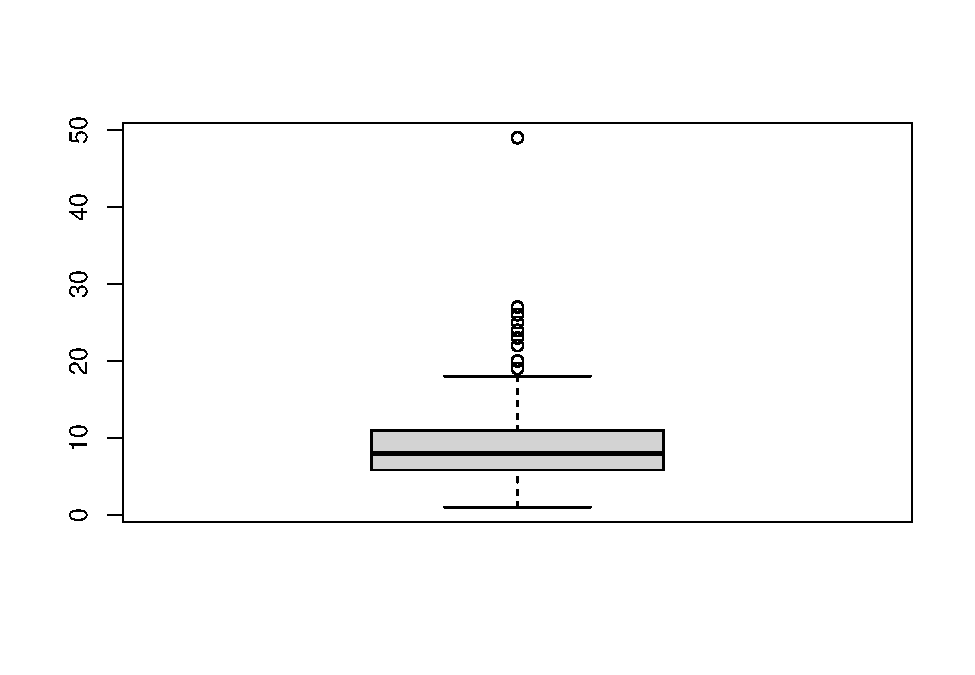
\includegraphics{PRAC2_Limpieza_Analisis_Datos---Sales_files/figure-latex/unnamed-chunk-15-1.pdf}

\begin{Shaded}
\begin{Highlighting}[]
\KeywordTok{boxplot.stats}\NormalTok{(SalesSummerObj}\OperatorTok{$}\NormalTok{price)}\OperatorTok{$}\NormalTok{out}
\end{Highlighting}
\end{Shaded}

\begin{verbatim}
##  [1] 20 22 19 19 19 20 24 22 49 19 23 22 20 25 19 26 20 19 27
\end{verbatim}

Vemos un único valor significativamente elevado (49). Vamos a
considerarlo como outlier y eliminamos el registro que lo contiene del
conjunto de datos.

\begin{Shaded}
\begin{Highlighting}[]
\NormalTok{SalesSummerObj <-}\StringTok{ }\NormalTok{SalesSummerObj[}\OperatorTok{!}\NormalTok{(SalesSummerObj}\OperatorTok{$}\NormalTok{price }\OperatorTok{==}\StringTok{ }\DecValTok{49}\NormalTok{),]}
\end{Highlighting}
\end{Shaded}

\begin{Shaded}
\begin{Highlighting}[]
\KeywordTok{boxplot}\NormalTok{(SalesSummerObj}\OperatorTok{$}\NormalTok{retail_price)}
\end{Highlighting}
\end{Shaded}

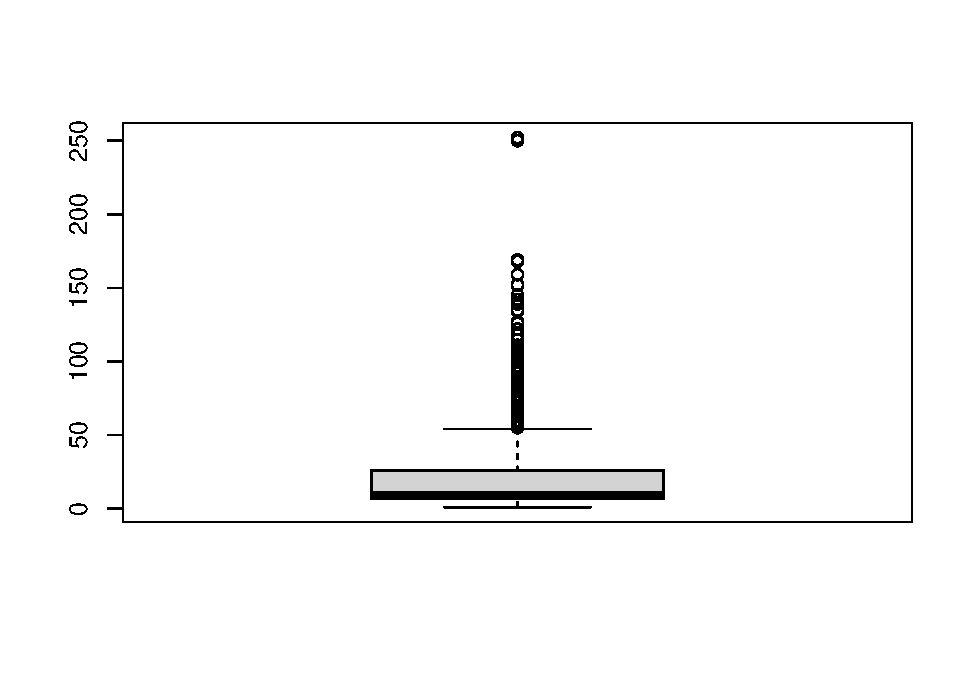
\includegraphics{PRAC2_Limpieza_Analisis_Datos---Sales_files/figure-latex/unnamed-chunk-17-1.pdf}

\begin{Shaded}
\begin{Highlighting}[]
\KeywordTok{boxplot.stats}\NormalTok{(SalesSummerObj}\OperatorTok{$}\NormalTok{retail_price)}\OperatorTok{$}\NormalTok{out}
\end{Highlighting}
\end{Shaded}

\begin{verbatim}
##   [1]  84  81  76  81  68  56  60  56  68  67  92  92  65  67  85  59  56  76
##  [19]  56  84  76 115  89  84 145  59 169  56  76  65  84 101  89  56  59  84
##  [37]  59  88 118  57 104  81  89  60 118  75  84  59  58  75 134 115  59 106
##  [55] 108 152 106  85  72 159 108 159  68  76  56 140 168 168  85  81  85  75
##  [73]  59  59  84  76  68  59  93  84 122  85  75  72  84  86 127  70 140 159
##  [91] 159 127 100 126  97  58 250  85  85  68 118  92 109  85  55  84  58  84
## [109]  84 111  65  67  84  59  56  84  93  59  69  85  85  56 142  86  65  58
## [127]  66  76 102  59  83 105  59  59  68  84  56  55  84  58 152  56  85  85
## [145]  84 110 102  75  68  84  68  59 168 252 168  85  76  65  65 140 102  59
## [163]  67  68 102  60  84  84  85 102  59 135  65 107  93  59 252  83  68  85
## [181]  75  68  75 139  84  84  84  59 108  76  84  59  84  59  68 108 168  88
## [199]  76  76  64  84  87  72  76  92 134  56
\end{verbatim}

En la variable retail\_price existen dos valores extremos, pero al
tratarse de precios podemos considerarlos valores válidos así que no los
consideraremos outliers y no los eliminaremos del conjunto de datos.

\begin{Shaded}
\begin{Highlighting}[]
\KeywordTok{boxplot}\NormalTok{(SalesSummerObj}\OperatorTok{$}\NormalTok{units_sold)}
\end{Highlighting}
\end{Shaded}

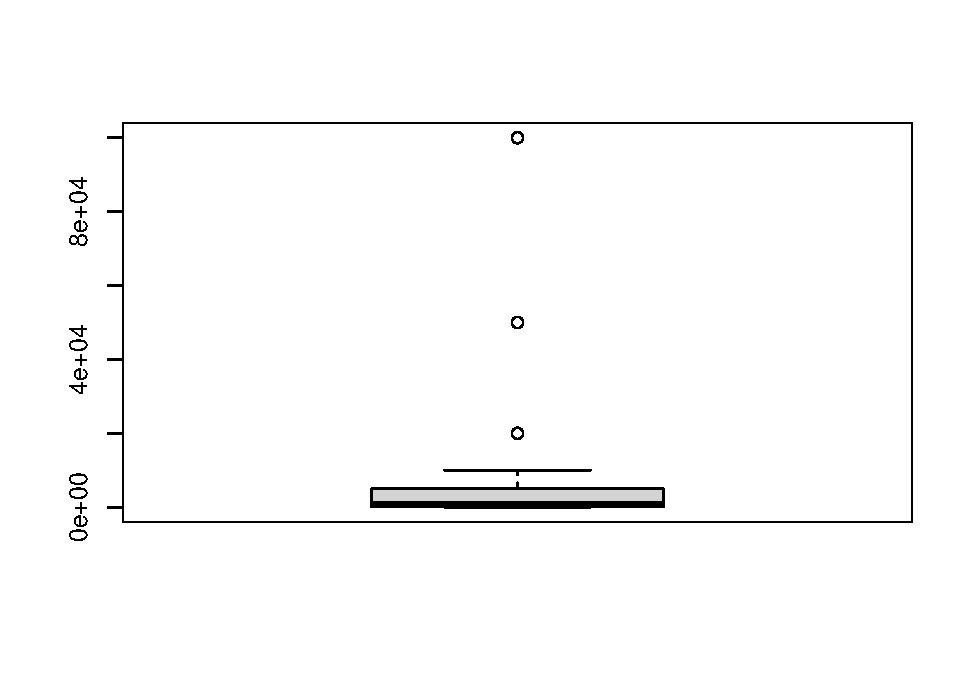
\includegraphics{PRAC2_Limpieza_Analisis_Datos---Sales_files/figure-latex/unnamed-chunk-18-1.pdf}

El mismo caso se repite con las unidades vendidas, pero estaríamos
hablando de una gran cantidad de unidades vendidas por encima de la
media del conjunto de datos. Estos valores pueden provocar que los
resultados en nuestro estudio se vean afectamos. Así que decidimos
eliminar dichos registros.

\begin{Shaded}
\begin{Highlighting}[]
\NormalTok{SalesSummerObj <-}\StringTok{ }\NormalTok{SalesSummerObj[}\OperatorTok{!}\NormalTok{(SalesSummerObj}\OperatorTok{$}\NormalTok{units_sold }\OperatorTok{>}\StringTok{ }\DecValTok{2000}\NormalTok{),]}
\end{Highlighting}
\end{Shaded}

\begin{Shaded}
\begin{Highlighting}[]
\KeywordTok{boxplot.stats}\NormalTok{(SalesSummerObj}\OperatorTok{$}\NormalTok{rating)}\OperatorTok{$}\NormalTok{out}
\end{Highlighting}
\end{Shaded}

\begin{verbatim}
##  [1] 1.50 2.00 2.00 2.00 2.00 1.00 2.00 2.25 2.00 2.00 1.00 2.33 2.00 2.44 2.00
## [16] 1.50 2.33 1.00 2.44
\end{verbatim}

Hablamos de un rating que va entre 1 y 5, y que ha sido calculado de
origen a partir de las otras variable rating. No vamos a efectuar
cambios sobre ellos. Tampoco vamos a realizar alteraciones sobre los
valores de los ratings 1-5.

\begin{Shaded}
\begin{Highlighting}[]
\KeywordTok{boxplot.stats}\NormalTok{(SalesSummerObj}\OperatorTok{$}\NormalTok{product_variation_inventory)}\OperatorTok{$}\NormalTok{out}
\end{Highlighting}
\end{Shaded}

\begin{verbatim}
## integer(0)
\end{verbatim}

\begin{Shaded}
\begin{Highlighting}[]
\KeywordTok{boxplot.stats}\NormalTok{(SalesSummerObj}\OperatorTok{$}\NormalTok{inventory_total)}\OperatorTok{$}\NormalTok{out}
\end{Highlighting}
\end{Shaded}

\begin{verbatim}
## [1] 40 36 30  9 24 37 38  2
\end{verbatim}

Se trata de valores de inventario que no vamos a categorizar como
outliers.

\begin{Shaded}
\begin{Highlighting}[]
\KeywordTok{boxplot.stats}\NormalTok{(SalesSummerObj}\OperatorTok{$}\NormalTok{merchant_rating)}\OperatorTok{$}\NormalTok{out}
\end{Highlighting}
\end{Shaded}

\begin{verbatim}
##  [1] 3.298507 3.186047 3.473684 3.409471 3.034483 5.000000 2.941176 3.417722
##  [9] 3.409471 3.381868 3.038961 3.475584 2.333333 3.464286 3.338290 3.381868
## [17] 4.577519 3.187500 3.186047 3.187500 3.367133 3.250000 3.422535 3.475584
## [25] 3.000000
\end{verbatim}

Se trata de un rating que va entre 2.333 y 5, no vamos a caterogizarlos
como outliers

\hypertarget{exportaciuxf3n-de-los-datos-preprocesados}{%
\subsection{2.3.4 - Exportación de los datos
preprocesados}\label{exportaciuxf3n-de-los-datos-preprocesados}}

Exportamos los datos preprocesados a un fichero .csv

\begin{Shaded}
\begin{Highlighting}[]
\CommentTok{# Exportación de los datos preprocesados a un fichero .csv}

\KeywordTok{write.csv}\NormalTok{(SalesSummerObj,}\StringTok{"spwrap_2020_08_data_clean.csv"}\NormalTok{)}
\end{Highlighting}
\end{Shaded}

\hypertarget{factorizaciuxf3n-y-niveles-de-las-variables-cuantitativas}{%
\subsection{2.3.5 - Factorización y niveles de las variables
cuantitativas}\label{factorizaciuxf3n-y-niveles-de-las-variables-cuantitativas}}

Vamos a factorizar la variable product\_color.

\begin{Shaded}
\begin{Highlighting}[]
\CommentTok{# Convertimos en factor y vemos sus niveles}

\KeywordTok{levels}\NormalTok{(}\KeywordTok{factor}\NormalTok{(SalesSummerObj}\OperatorTok{$}\NormalTok{product_color))}
\end{Highlighting}
\end{Shaded}

\begin{verbatim}
##  [1] "applegreen"          "apricot"             "army"               
##  [4] "army green"          "beige"               "black"              
##  [7] "black & blue"        "black & green"       "black & white"      
## [10] "black & yellow"      "blue"                "brown"              
## [13] "brown & yellow"      "camel"               "camouflage"         
## [16] "claret"              "coffee"              "coolblack"          
## [19] "coralred"            "darkblue"            "darkgreen"          
## [22] "dustypink"           "floral"              "fluorescentgreen"   
## [25] "gray"                "gray & white"        "green"              
## [28] "grey"                "greysnakeskinprint"  "khaki"              
## [31] "lakeblue"            "leopard"             "leopardprint"       
## [34] "lightblue"           "lightgray"           "lightgreen"         
## [37] "lightgrey"           "lightpink"           "lightpurple"        
## [40] "lightred"            "lightyellow"         "mintgreen"          
## [43] "multicolor"          "navy"                "navyblue"           
## [46] "no color"            "offblack"            "offwhite"           
## [49] "orange"              "orange-red"          "orange & camouflage"
## [52] "pink"                "pink & black"        "pink & blue"        
## [55] "pink & grey"         "pink & white"        "prussianblue"       
## [58] "purple"              "rainbow"             "red"                
## [61] "red & blue"          "rose"                "rosered"            
## [64] "silver"              "skyblue"             "tan"                
## [67] "violet"              "white"               "white & black"      
## [70] "white & green"       "whitefloral"         "wine"               
## [73] "winered"             "winered & yellow"    "yellow"
\end{verbatim}

Factorizamos los valores para dicha variable

\begin{Shaded}
\begin{Highlighting}[]
\NormalTok{SalesSummerObj}\OperatorTok{$}\NormalTok{product_color <-}\StringTok{ }\KeywordTok{as.numeric}\NormalTok{(}\KeywordTok{factor}\NormalTok{(SalesSummerObj}\OperatorTok{$}\NormalTok{product_color))}
\end{Highlighting}
\end{Shaded}

\hypertarget{anuxe1lisis-de-los-datos}{%
\section{2.4 - ANÁLISIS DE LOS DATOS}\label{anuxe1lisis-de-los-datos}}

\hypertarget{selecciuxf3n-de-grupos-de-datos}{%
\subsection{2.4.2 - Selección de grupos de
datos}\label{selecciuxf3n-de-grupos-de-datos}}

Seleccionamos un conjunto inicial de grupos de datos que nos pueden
resultar interesantes de analizar y/o comparar.

\textbf{Agrupación por utilización de anuncios uses\_ad\_boosts (0/1)}

\begin{Shaded}
\begin{Highlighting}[]
\NormalTok{SalesSummerObj.uses.ad.boosts.cero <-}\StringTok{ }\NormalTok{SalesSummerObj }\OperatorTok\StringTok{ }\KeywordTok{filter}\NormalTok{(uses_ad_boosts }\OperatorTok{==}\StringTok{ "0"}\NormalTok{)}
\NormalTok{SalesSummerObj.uses.ad.boosts.uno <-}\StringTok{ }\NormalTok{SalesSummerObj }\OperatorTok\StringTok{ }\KeywordTok{filter}\NormalTok{(uses_ad_boosts }\OperatorTok{==}\StringTok{ "1"}\NormalTok{)}
\end{Highlighting}
\end{Shaded}

\textbf{Agrupación por insignia local product}

\begin{Shaded}
\begin{Highlighting}[]
\NormalTok{SalesSummerObj.badget.localproduct.cero <-}\StringTok{ }\NormalTok{SalesSummerObj }\OperatorTok\StringTok{ }\KeywordTok{filter}\NormalTok{(badge_local_product}\OperatorTok{==}\StringTok{ "0"}\NormalTok{)}
\NormalTok{SalesSummerObj.badget.localproduct.uno <-}\StringTok{ }\NormalTok{SalesSummerObj }\OperatorTok\StringTok{ }\KeywordTok{filter}\NormalTok{(badge_local_product}\OperatorTok{==}\StringTok{ "1"}\NormalTok{)}
\end{Highlighting}
\end{Shaded}

\textbf{Agrupación por insignia product quality}

\begin{Shaded}
\begin{Highlighting}[]
\NormalTok{SalesSummerObj.badget.productquality.cero <-}\StringTok{ }\NormalTok{SalesSummerObj }\OperatorTok\StringTok{ }\KeywordTok{filter}\NormalTok{(badge_product_quality}\OperatorTok{==}\StringTok{ "0"}\NormalTok{)}
\NormalTok{SalesSummerObj.badget.productquality.uno <-}\StringTok{ }\NormalTok{SalesSummerObj }\OperatorTok\StringTok{ }\KeywordTok{filter}\NormalTok{(badge_product_quality }\OperatorTok{==}\StringTok{ "1"}\NormalTok{)}
\end{Highlighting}
\end{Shaded}

\textbf{Agrupación por insignia fast shipping}

\begin{Shaded}
\begin{Highlighting}[]
\NormalTok{SalesSummerObj.badget.fastshipping.cero <-}\StringTok{ }\NormalTok{SalesSummerObj }\OperatorTok\StringTok{ }\KeywordTok{filter}\NormalTok{(badge_fast_shipping }\OperatorTok{==}\StringTok{ "0"}\NormalTok{)}
\NormalTok{SalesSummerObj.badget.fastshipping.uno <-}\StringTok{ }\NormalTok{SalesSummerObj }\OperatorTok\StringTok{ }\KeywordTok{filter}\NormalTok{(badge_fast_shipping }\OperatorTok{==}\StringTok{ "1"}\NormalTok{)}
\end{Highlighting}
\end{Shaded}

\textbf{Agrupación por shipping express}

\begin{Shaded}
\begin{Highlighting}[]
\NormalTok{SalesSummerObj.shipping.express.cero <-}\StringTok{ }\NormalTok{SalesSummerObj }\OperatorTok\StringTok{ }\KeywordTok{filter}\NormalTok{(shipping_is_express }\OperatorTok{==}\StringTok{ "0"}\NormalTok{)}
\NormalTok{SalesSummerObj.shipping.express.uno <-}\StringTok{ }\NormalTok{SalesSummerObj }\OperatorTok\StringTok{ }\KeywordTok{filter}\NormalTok{(shipping_is_express }\OperatorTok{==}\StringTok{ "1"}\NormalTok{)}
\end{Highlighting}
\end{Shaded}

\textbf{Agrupación por intervalos de rating}

rating \textless=1.5 -\textgreater{} Intervalo 1 rating \textgreater1.5
and \textless{} 2.5 -\textgreater{} Intervalo 2 rating \textgreater=2.5
and \textless{} 3.5 -\textgreater{} Intervalo 3 rating \textgreater=3.5
and \textless{} 4.5 -\textgreater{} Intervalo 4 rating \textgreater= 4.5
-\textgreater{} Intervalo 5

Para ello crearemos una variable rating\_interval donde asignaremos el
valor 1 a 5 dependiendo del rango de valores definidos:

\begin{Shaded}
\begin{Highlighting}[]
\NormalTok{SalesSummerObj <-}\StringTok{ }\KeywordTok{cbind}\NormalTok{(SalesSummerObj,}\DataTypeTok{rating_interval=}\KeywordTok{c}\NormalTok{(}\KeywordTok{as.integer}\NormalTok{(}\DecValTok{0}\NormalTok{)))}

\NormalTok{SalesSummerObj}\OperatorTok{$}\NormalTok{rating_interval[SalesSummerObj}\OperatorTok{$}\NormalTok{rating }\OperatorTok{<=}\StringTok{ }\FloatTok{1.5}\NormalTok{ ] <-}\StringTok{ }\DecValTok{1}
\NormalTok{SalesSummerObj}\OperatorTok{$}\NormalTok{rating_interval[SalesSummerObj}\OperatorTok{$}\NormalTok{rating }\OperatorTok{>}\StringTok{ }\FloatTok{1.5} \OperatorTok{&}\StringTok{ }\NormalTok{SalesSummerObj}\OperatorTok{$}\NormalTok{rating }\OperatorTok{<}\StringTok{ }\FloatTok{2.5}\NormalTok{  ] <-}\StringTok{ }\DecValTok{2}
\NormalTok{SalesSummerObj}\OperatorTok{$}\NormalTok{rating_interval[SalesSummerObj}\OperatorTok{$}\NormalTok{rating }\OperatorTok{>=}\FloatTok{2.5} \OperatorTok{&}\StringTok{ }\NormalTok{SalesSummerObj}\OperatorTok{$}\NormalTok{rating }\OperatorTok{<}\StringTok{ }\FloatTok{3.5}\NormalTok{  ] <-}\StringTok{ }\DecValTok{3}
\NormalTok{SalesSummerObj}\OperatorTok{$}\NormalTok{rating_interval[SalesSummerObj}\OperatorTok{$}\NormalTok{rating }\OperatorTok{>=}\FloatTok{3.5} \OperatorTok{&}\StringTok{ }\NormalTok{SalesSummerObj}\OperatorTok{$}\NormalTok{rating }\OperatorTok{<}\StringTok{ }\FloatTok{4.5}\NormalTok{  ] <-}\StringTok{ }\DecValTok{4}
\NormalTok{SalesSummerObj}\OperatorTok{$}\NormalTok{rating_interval[SalesSummerObj}\OperatorTok{$}\NormalTok{rating }\OperatorTok{>=}\FloatTok{4.5}\NormalTok{] <-}\StringTok{ }\DecValTok{5}
\end{Highlighting}
\end{Shaded}

\begin{Shaded}
\begin{Highlighting}[]
\NormalTok{SalesSummerObj.rating.interval.uno <-}\StringTok{ }\NormalTok{SalesSummerObj }\OperatorTok\StringTok{ }\KeywordTok{filter}\NormalTok{(SalesSummerObj}\OperatorTok{$}\NormalTok{rating_interval }\OperatorTok{==}\StringTok{ "1"}\NormalTok{)}
\NormalTok{SalesSummerObj.rating.interval.dos <-}\StringTok{ }\NormalTok{SalesSummerObj }\OperatorTok\StringTok{ }\KeywordTok{filter}\NormalTok{(SalesSummerObj}\OperatorTok{$}\NormalTok{rating_interval }\OperatorTok{==}\StringTok{ "2"}\NormalTok{)}
\NormalTok{SalesSummerObj.rating.interval.tres <-}\StringTok{ }\NormalTok{SalesSummerObj }\OperatorTok\StringTok{ }\KeywordTok{filter}\NormalTok{(SalesSummerObj}\OperatorTok{$}\NormalTok{rating_interval }\OperatorTok{==}\StringTok{ "3"}\NormalTok{)}
\NormalTok{SalesSummerObj.rating.interval.cuatro <-}\StringTok{ }\NormalTok{SalesSummerObj }\OperatorTok\StringTok{ }\KeywordTok{filter}\NormalTok{(SalesSummerObj}\OperatorTok{$}\NormalTok{rating_interval }\OperatorTok{==}\StringTok{ "4"}\NormalTok{)}
\NormalTok{SalesSummerObj.rating.interval.cinco <-}\StringTok{ }\NormalTok{SalesSummerObj }\OperatorTok\StringTok{ }\KeywordTok{filter}\NormalTok{(SalesSummerObj}\OperatorTok{$}\NormalTok{rating_interval }\OperatorTok{==}\StringTok{ "5"}\NormalTok{)}
\end{Highlighting}
\end{Shaded}

*** Agrupación por tallas grandes y pequeñas ***

Añadimos una variable size\_category inicializada con valor EC (Empty
Category)

\begin{Shaded}
\begin{Highlighting}[]
\NormalTok{SalesSummerObj <-}\StringTok{ }\KeywordTok{cbind}\NormalTok{(SalesSummerObj,}\DataTypeTok{size_category=}\KeywordTok{c}\NormalTok{(}\StringTok{"EC"}\NormalTok{))}
\end{Highlighting}
\end{Shaded}

Seteamos la nueva variable en funcion de tallas pequeñas (SS) o grandes
(HS)

\begin{Shaded}
\begin{Highlighting}[]
\NormalTok{SalesSummerObj}\OperatorTok{$}\NormalTok{size_category[SalesSummerObj}\OperatorTok{$}\NormalTok{product_variation_size_id }\OperatorTok{==}\StringTok{ "3XS"} \OperatorTok{|}\StringTok{ }
\NormalTok{SalesSummerObj}\OperatorTok{$}\NormalTok{product_variation_size_id }\OperatorTok{==}\StringTok{ "2XS"} \OperatorTok{|}\StringTok{ }\NormalTok{SalesSummerObj}\OperatorTok{$}\NormalTok{product_variation_size_id }\OperatorTok{==}\StringTok{ "XS"} \OperatorTok{|}\StringTok{ }
\NormalTok{SalesSummerObj}\OperatorTok{$}\NormalTok{product_variation_size_id }\OperatorTok{==}\StringTok{ "S"}\NormalTok{] <-}\StringTok{ "SS"}

\NormalTok{SalesSummerObj}\OperatorTok{$}\NormalTok{size_category[SalesSummerObj}\OperatorTok{$}\NormalTok{product_variation_size_id }\OperatorTok{==}\StringTok{ "XL"} \OperatorTok{|}\StringTok{ }
\NormalTok{SalesSummerObj}\OperatorTok{$}\NormalTok{product_variation_size_id }\OperatorTok{==}\StringTok{ "2XL"} \OperatorTok{|}\NormalTok{SalesSummerObj}\OperatorTok{$}\NormalTok{product_variation_size_id }\OperatorTok{==}\StringTok{  "3XL"} \OperatorTok{|}\StringTok{ }
\NormalTok{SalesSummerObj}\OperatorTok{$}\NormalTok{product_variation_size_id }\OperatorTok{==}\StringTok{ "4XL"} \OperatorTok{|}\StringTok{ }\NormalTok{SalesSummerObj}\OperatorTok{$}\NormalTok{product_variation_size_id }\OperatorTok{==}\StringTok{ "5XL"} \OperatorTok{|}\StringTok{ }
\NormalTok{SalesSummerObj}\OperatorTok{$}\NormalTok{product_variation_size_id }\OperatorTok{==}\StringTok{ "6XL"}\NormalTok{] <-}\StringTok{ "HS"}
\end{Highlighting}
\end{Shaded}

\hypertarget{comprobaciuxf3n-de-normalidad-y-homogeneidad-de-la-varianza}{%
\subsection{2.4.3 - Comprobación de normalidad y homogeneidad de la
varianza}\label{comprobaciuxf3n-de-normalidad-y-homogeneidad-de-la-varianza}}

Para la comprobación de que los valores que toman nuestras variables
cuantitativas provienen de una población distribuida normalmente,
utilizaremos la prueba de normalidad deShapiro. Se comprueba si el
p-valor es superior al nivel de significación prefijado alfa = 0.05. Si
esto se cumple, entonces se considera que variable en cuestión sigue una
distribución normal.

\begin{Shaded}
\begin{Highlighting}[]
\NormalTok{alpha =}\StringTok{ }\FloatTok{0.05}

\NormalTok{col.names =}\StringTok{ }\KeywordTok{colnames}\NormalTok{(SalesSummerObj)}

\ControlFlowTok{for}\NormalTok{ (i }\ControlFlowTok{in} \DecValTok{1}\OperatorTok{:}\KeywordTok{ncol}\NormalTok{(SalesSummerObj)) }
\NormalTok{  \{}
    \ControlFlowTok{if}\NormalTok{ (i }\OperatorTok{==}\StringTok{ }\DecValTok{1}\NormalTok{) }\KeywordTok{cat}\NormalTok{(}\StringTok{"Variables que no siguen una distribución normal:}\CharTok{\textbackslash{}n}\StringTok{"}\NormalTok{)}
      \ControlFlowTok{if}\NormalTok{ (}\KeywordTok{is.integer}\NormalTok{(SalesSummerObj[,i]) }\OperatorTok{|}\StringTok{ }\KeywordTok{is.numeric}\NormalTok{(SalesSummerObj[,i])) }
\NormalTok{        \{}
\NormalTok{          p_val =}\StringTok{ }\KeywordTok{shapiro.test}\NormalTok{(SalesSummerObj[,i])}\OperatorTok{$}\NormalTok{p.value}
          \ControlFlowTok{if}\NormalTok{ (p_val }\OperatorTok{<}\StringTok{ }\NormalTok{alpha) \{}
                              \KeywordTok{cat}\NormalTok{(col.names[i])}
                              \ControlFlowTok{if}\NormalTok{ (i }\OperatorTok{<}\StringTok{ }\KeywordTok{ncol}\NormalTok{(SalesSummerObj) }\OperatorTok{-}\StringTok{ }\DecValTok{1}\NormalTok{) }\KeywordTok{cat}\NormalTok{(}\StringTok{", "}\NormalTok{)}
                              \ControlFlowTok{if}\NormalTok{ (i }\OperatorTok\StringTok{ }\DecValTok{2} \OperatorTok{==}\StringTok{ }\DecValTok{0}\NormalTok{) }\KeywordTok{cat}\NormalTok{(}\StringTok{"}\CharTok{\textbackslash{}n}\StringTok{"}\NormalTok{)}
\NormalTok{                            \}}
\NormalTok{        \}}
\NormalTok{  \}}
\end{Highlighting}
\end{Shaded}

\begin{verbatim}
## Variables que no siguen una distribución normal:
## price, retail_price, 
## units_sold, uses_ad_boosts, 
## rating, rating_count, 
## rating_five_count, rating_four_count, 
## rating_three_count, rating_two_count, 
## rating_one_count, badges_count, 
## badge_local_product, badge_product_quality, 
## badge_fast_shipping, product_color, product_variation_inventory, 
## shipping_is_express, countries_shipped_to, 
## inventory_total, merchant_rating, 
## rating_interval
\end{verbatim}

Podemos comprobarlo gráficamente por ejemplo con la variable price.

\begin{Shaded}
\begin{Highlighting}[]
\KeywordTok{ggplot}\NormalTok{(}\DataTypeTok{data =}\NormalTok{ SalesSummerObj, }\KeywordTok{aes}\NormalTok{(}\DataTypeTok{x =}\NormalTok{ price)) }\OperatorTok{+}
\StringTok{  }\KeywordTok{geom_histogram}\NormalTok{(}\KeywordTok{aes}\NormalTok{(}\DataTypeTok{y =}\NormalTok{ ..density..,}\DataTypeTok{fill =}\NormalTok{ ..count..)) }\OperatorTok{+}
\StringTok{  }\KeywordTok{stat_function}\NormalTok{(}\DataTypeTok{fun =}\NormalTok{ dnorm, }\DataTypeTok{colour =} \StringTok{"firebrick"}\NormalTok{,}
                \DataTypeTok{args =} \KeywordTok{list}\NormalTok{(}\DataTypeTok{mean =} \KeywordTok{mean}\NormalTok{(SalesSummerObj}\OperatorTok{$}\NormalTok{price),}
                            \DataTypeTok{sd =} \KeywordTok{sd}\NormalTok{(SalesSummerObj}\OperatorTok{$}\NormalTok{price))) }\OperatorTok{+}
\StringTok{  }\KeywordTok{ggtitle}\NormalTok{(}\StringTok{"Histograma + curva normal teórica (price)"}\NormalTok{)}
\end{Highlighting}
\end{Shaded}

\begin{verbatim}
## `stat_bin()` using `bins = 30`. Pick better value with `binwidth`.
\end{verbatim}

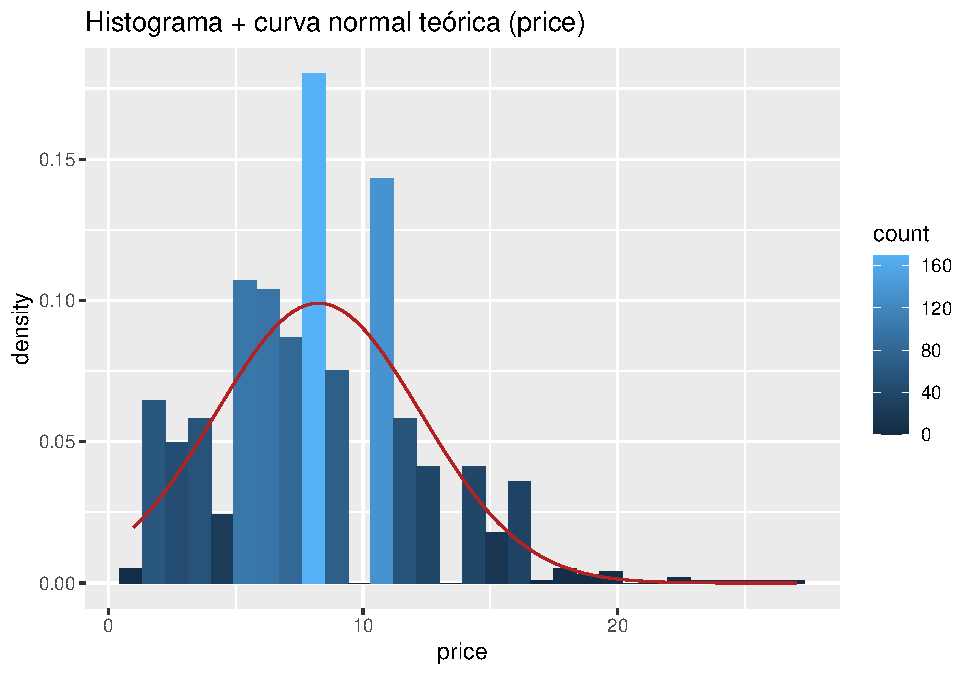
\includegraphics{PRAC2_Limpieza_Analisis_Datos---Sales_files/figure-latex/unnamed-chunk-37-1.pdf}

\begin{Shaded}
\begin{Highlighting}[]
\KeywordTok{qplot}\NormalTok{(price, }\DataTypeTok{data =}\NormalTok{ SalesSummerObj,}\DataTypeTok{geom=}\StringTok{"density"}\NormalTok{)}\OperatorTok{+}\StringTok{ }\KeywordTok{geom_vline}\NormalTok{(}\DataTypeTok{xintercept =} \KeywordTok{mean}\NormalTok{(SalesSummerObj}\OperatorTok{$}\NormalTok{price),}
\DataTypeTok{color=}\StringTok{"red"}\NormalTok{)}\OperatorTok{+}\StringTok{ }\KeywordTok{geom_vline}\NormalTok{(}\DataTypeTok{xintercept =} \KeywordTok{median}\NormalTok{(SalesSummerObj}\OperatorTok{$}\NormalTok{price), }\DataTypeTok{color=}\StringTok{"blue"}\NormalTok{)}
\end{Highlighting}
\end{Shaded}

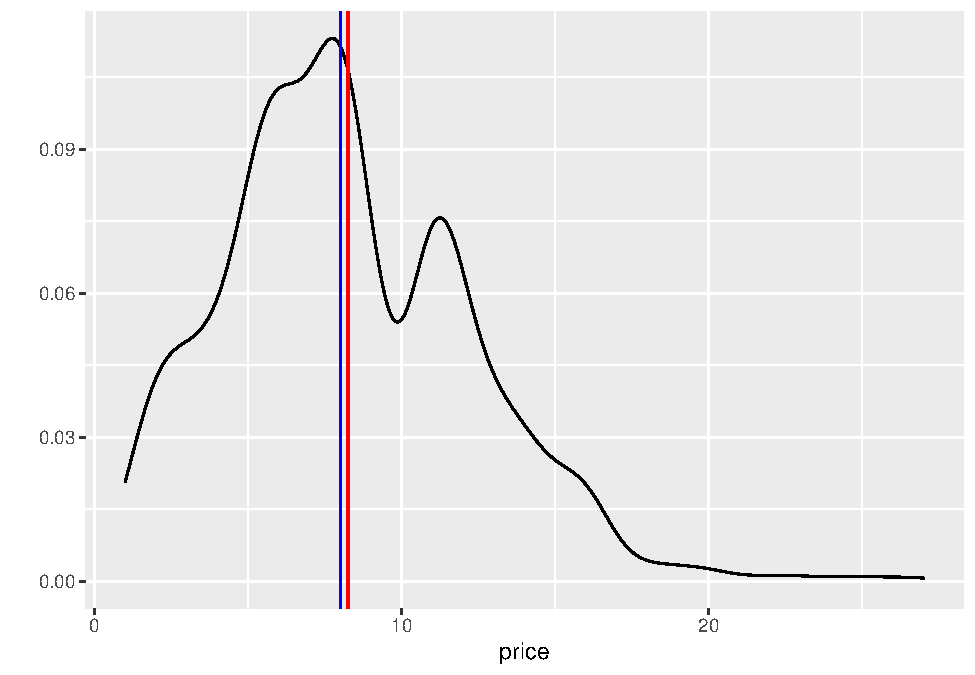
\includegraphics{PRAC2_Limpieza_Analisis_Datos---Sales_files/figure-latex/unnamed-chunk-38-1.pdf}

\textbf{Ninguna de las variables seleccionadas es normal}

Seguidamente, pasamos a estudiar la homogeneidad de varianzas.

Como ninguna de las variables es normal aplicaremos el test de Levene
entre price y las variables que vamos a utilizar. Este test prueba la
hipótesis nula de que las varianzas poblacionales son iguales.

\begin{Shaded}
\begin{Highlighting}[]
\KeywordTok{leveneTest}\NormalTok{(price }\OperatorTok{~}\StringTok{ }\KeywordTok{factor}\NormalTok{(SalesSummerObj}\OperatorTok{$}\NormalTok{uses_ad_boosts), SalesSummerObj, }\DataTypeTok{center=}\NormalTok{median)}
\end{Highlighting}
\end{Shaded}

\begin{verbatim}
## Levene's Test for Homogeneity of Variance (center = median)
##         Df F value    Pr(>F)    
## group    1   11.32 0.0007944 ***
##       1050                      
## ---
## Signif. codes:  0 '***' 0.001 '**' 0.01 '*' 0.05 '.' 0.1 ' ' 1
\end{verbatim}

\begin{Shaded}
\begin{Highlighting}[]
\KeywordTok{leveneTest}\NormalTok{(price }\OperatorTok{~}\StringTok{ }\KeywordTok{factor}\NormalTok{(SalesSummerObj}\OperatorTok{$}\NormalTok{badge_local_product), SalesSummerObj, }\DataTypeTok{center=}\NormalTok{median)}
\end{Highlighting}
\end{Shaded}

\begin{verbatim}
## Levene's Test for Homogeneity of Variance (center = median)
##         Df F value Pr(>F)
## group    1    0.91 0.3403
##       1050
\end{verbatim}

\begin{Shaded}
\begin{Highlighting}[]
\KeywordTok{leveneTest}\NormalTok{(price }\OperatorTok{~}\StringTok{ }\KeywordTok{factor}\NormalTok{(SalesSummerObj}\OperatorTok{$}\NormalTok{badge_product_quality), SalesSummerObj, }\DataTypeTok{center=}\NormalTok{median)}
\end{Highlighting}
\end{Shaded}

\begin{verbatim}
## Levene's Test for Homogeneity of Variance (center = median)
##         Df F value Pr(>F)
## group    1  2.0329 0.1542
##       1050
\end{verbatim}

\begin{Shaded}
\begin{Highlighting}[]
\KeywordTok{leveneTest}\NormalTok{(price }\OperatorTok{~}\StringTok{ }\KeywordTok{factor}\NormalTok{(SalesSummerObj}\OperatorTok{$}\NormalTok{badge_fast_shipping), SalesSummerObj, }\DataTypeTok{center=}\NormalTok{median)}
\end{Highlighting}
\end{Shaded}

\begin{verbatim}
## Levene's Test for Homogeneity of Variance (center = median)
##         Df F value    Pr(>F)    
## group    1  12.118 0.0005198 ***
##       1050                      
## ---
## Signif. codes:  0 '***' 0.001 '**' 0.01 '*' 0.05 '.' 0.1 ' ' 1
\end{verbatim}

\begin{Shaded}
\begin{Highlighting}[]
\KeywordTok{leveneTest}\NormalTok{(price }\OperatorTok{~}\StringTok{ }\KeywordTok{factor}\NormalTok{(SalesSummerObj}\OperatorTok{$}\NormalTok{shipping_is_express), SalesSummerObj, }\DataTypeTok{center=}\NormalTok{median)}
\end{Highlighting}
\end{Shaded}

\begin{verbatim}
## Levene's Test for Homogeneity of Variance (center = median)
##         Df F value Pr(>F)
## group    1  0.2407 0.6238
##       1050
\end{verbatim}

\begin{Shaded}
\begin{Highlighting}[]
\KeywordTok{leveneTest}\NormalTok{(price }\OperatorTok{~}\StringTok{ }\KeywordTok{factor}\NormalTok{(SalesSummerObj}\OperatorTok{$}\NormalTok{rating_interval), SalesSummerObj, }\DataTypeTok{center=}\NormalTok{median)}
\end{Highlighting}
\end{Shaded}

\begin{verbatim}
## Levene's Test for Homogeneity of Variance (center = median)
##         Df F value Pr(>F)
## group    4  0.5301 0.7136
##       1047
\end{verbatim}

\begin{Shaded}
\begin{Highlighting}[]
\KeywordTok{leveneTest}\NormalTok{(price }\OperatorTok{~}\StringTok{ }\KeywordTok{factor}\NormalTok{(SalesSummerObj}\OperatorTok{$}\NormalTok{origin_country), SalesSummerObj, }\DataTypeTok{center=}\NormalTok{median)}
\end{Highlighting}
\end{Shaded}

\begin{verbatim}
## Levene's Test for Homogeneity of Variance (center = median)
##         Df F value Pr(>F)
## group    6  1.4923 0.1774
##       1045
\end{verbatim}

Si el P-valor resultante de la prueba de Levene es inferior a un cierto
nivel de significación (típicamente 0.05), es poco probable que las
diferencias obtenidas en las variaciones de la muestra se hayan
producido sobre la base de un muestreo aleatorio de una población con
varianzas iguales. Por lo tanto, la hipótesis nula de igualdad de
varianzas se rechaza y se concluye que hay una diferencia entre las
variaciones en la población.

Los resultados indican que \textbf{existen diferencias significativas}
en las varianzas de los grupos creados por los valores de
uses\_ad\_boosts y badge\_fast\_shipping. Para el resto de variables a
estudiar, \textbf{no hay diferencias significativas} entre las varianzas
de los grupos, es decir existe homogeneidad de varianza u
homocedasticidad.

\hypertarget{aplicaciuxf3n-de-pruebas-estaduxedsticas}{%
\subsection{2.4.4 - Aplicación de pruebas
estadísticas}\label{aplicaciuxf3n-de-pruebas-estaduxedsticas}}

\hypertarget{estudio-de-la-correlaciuxf3n-test-de-spearman}{%
\subsubsection{2.4.4.1 - Estudio de la Correlación / Test de
Spearman}\label{estudio-de-la-correlaciuxf3n-test-de-spearman}}

En primer lugar, procedemos a realizar un análisis de correlación entre
las distintas variables para determinar cuáles de ellas ejercen una
mayor influencia sobre el precio del artículo. Para ello, se utilizará
el coeficiente de correlación de Spearman, puesto que hemos visto que
tenemos datos que no siguen una distribución normal.

\begin{Shaded}
\begin{Highlighting}[]
\KeywordTok{print}\NormalTok{(corr_matrix)}
\end{Highlighting}
\end{Shaded}

\begin{verbatim}
##                                estimate      p-value
## retail_price                 0.54914958 6.556328e-84
## units_sold                   0.07772473 1.167610e-02
## uses_ad_boosts              -0.10989721 3.555528e-04
## rating                       0.06644395 3.116974e-02
## rating_count                 0.19701440 1.150286e-10
## rating_five_count            0.20422930 2.280884e-11
## rating_four_count            0.20286444 3.112111e-11
## rating_three_count           0.18214944 2.668989e-09
## rating_two_count             0.16595843 6.164154e-08
## rating_one_count             0.17935725 4.684162e-09
## badges_count                 0.02374221 4.417384e-01
## badge_local_product          0.06299565 4.106870e-02
## badge_product_quality        0.01130843 7.140967e-01
## badge_fast_shipping          0.01850128 5.488938e-01
## product_color               -0.02341265 4.481039e-01
## product_variation_inventory  0.38873242 2.789456e-39
## shipping_is_express          0.03751469 2.240789e-01
## countries_shipped_to        -0.02096194 4.970382e-01
## inventory_total             -0.05691424 6.499553e-02
## merchant_rating              0.06539757 3.393109e-02
## rating_interval              0.05781690 6.084722e-02
\end{verbatim}

Los grados de correlación de las variables son tanto más altos, cuanto
más cerca están de -1 o de 1. Teniendo esto en cuenta, la variable más
relevante en la fijación del precio es el precio de retail
(retail\_price), seguida de product\_variation\_inventory, y las
variables de rating\_*\_count. De cualquier forma, no hay ninguna
variable que este correlacionada de forma fuerte con la variable price,
ya que ninguna está por encima de 0.8

El valor P es la probabilidad de que hubiera encontrado el resultado
actual si el coeficiente de correlación fuera cero (hipótesis nula). Si
esta probabilidad es menor que el 5\% convencional (P \textless0.05), el
coeficiente de correlación se denomina estadísticamente significativo,
por lo que podemos concluir que, el coeficiente de correlación entre
retail\_price y price (0.5) es estadísticamente significativo, lo mismo
sucede para las variables rating\_*\_count.

El valor del coeficiente positivo, indica una correlación positiva, es
decir, cuanto mayor es el precio de retail, mayor es el precio del
producto.

\hypertarget{contraste-de-hipuxf3tesis}{%
\subsubsection{2.4.4.2 - Contraste de
Hipótesis}\label{contraste-de-hipuxf3tesis}}

\textbf{\emph{Determinar si el precio es superior dependiendo del
rating\_interval del producto}}

Para ello utilizaremos dos muestras: una cuando la variable
rating\_interval del producto es cinco (rating \textgreater= 4.5) y otra
cuando dicha variable es uno (rating \textless= 1.5)***

Para realizar este tipo de tests paramétricos, es preciso que los datos
sean normales, si la muestra es de tamaño inferior a 30. En nuestro
caso, el contraste de hipótesis es aplicable ya que superamos dicho
valor.

Planteamos un contraste de Hipótesis unilateral sobre la diferencia de
medias:

\[
  H_{0}: \mu_{1} - \mu_{2} = 0
\]

\[
  H_{1}: \mu_{1} - \mu_{2} < 0
\] donde mu1 es la media de la población de la que se extrae la primera
muestra y mu2 es la media de la población de la que extrae la segunda.
Así, tomaremos alfa = 0.05.

\begin{Shaded}
\begin{Highlighting}[]
\KeywordTok{t.test}\NormalTok{(SalesSummerObj.rating.interval.tres}\OperatorTok{$}\NormalTok{price,SalesSummerObj.rating.interval.cinco}\OperatorTok{$}\NormalTok{price,}\DataTypeTok{alternative =} \StringTok{"less"}\NormalTok{)}
\end{Highlighting}
\end{Shaded}

\begin{verbatim}
## 
##  Welch Two Sample t-test
## 
## data:  SalesSummerObj.rating.interval.tres$price and SalesSummerObj.rating.interval.cinco$price
## t = 0.32364, df = 229.22, p-value = 0.6267
## alternative hypothesis: true difference in means is less than 0
## 95 percent confidence interval:
##       -Inf 0.8571741
## sample estimates:
## mean of x mean of y 
##  7.837907  7.697455
\end{verbatim}

Obtenemos un p-value mayor que el valor de significación, por lo que no
podemos rechazar la hipotésis nula. Por lo tanto no podemos concluir que
los artículos con un rating\_interval = 5 sean más caros que los que
tienen un rating\_interval = 1.

\textbf{\emph{Determinar si el precio es superior para los productos de
mayor calidad}}

Para ello utilizaremos dos muestras: una cuando la variable
badget\_product\_quality del producto es 1 y otra cuando dicha variable
es 0***

Aplicaremos el mismo test de hipótesis que en el caso anterior.

\begin{Shaded}
\begin{Highlighting}[]
\KeywordTok{t.test}\NormalTok{(SalesSummerObj.badget.productquality.cero}\OperatorTok{$}\NormalTok{price,SalesSummerObj.badget.productquality.uno}\OperatorTok{$}\NormalTok{price,}\DataTypeTok{alternative =} \StringTok{"less"}\NormalTok{)}
\end{Highlighting}
\end{Shaded}

\begin{verbatim}
## 
##  Welch Two Sample t-test
## 
## data:  SalesSummerObj.badget.productquality.cero$price and SalesSummerObj.badget.productquality.uno$price
## t = -0.20757, df = 65.383, p-value = 0.4181
## alternative hypothesis: true difference in means is less than 0
## 95 percent confidence interval:
##       -Inf 0.8313407
## sample estimates:
## mean of x mean of y 
##  8.244718  8.362833
\end{verbatim}

Obtenemos un p-value mayor que el valor de significación, por lo que no
podemos rechazar la hipotésis nula. Por lo tanto no podemos concluir que
los artículos catalogados de mayor calidad tengan un precio superior

\textbf{\emph{Determinar si el uso de anuncios incrementa al precio del
producto}}

Para ello utilizaremos dos muestras: una cuando la variable
uses\_ad\_boosts del producto es 1 y otra cuando dicha variable es 0***

Aplicaremos el mismo test de hipótesis que en el caso anterior.

\begin{Shaded}
\begin{Highlighting}[]
\KeywordTok{t.test}\NormalTok{(SalesSummerObj.uses.ad.boosts.cero}\OperatorTok{$}\NormalTok{price,SalesSummerObj.uses.ad.boosts.uno}\OperatorTok{$}\NormalTok{price,}\DataTypeTok{alternative =} \StringTok{"less"}\NormalTok{)}
\end{Highlighting}
\end{Shaded}

\begin{verbatim}
## 
##  Welch Two Sample t-test
## 
## data:  SalesSummerObj.uses.ad.boosts.cero$price and SalesSummerObj.uses.ad.boosts.uno$price
## t = 2.8237, df = 920.87, p-value = 0.9976
## alternative hypothesis: true difference in means is less than 0
## 95 percent confidence interval:
##      -Inf 1.132499
## sample estimates:
## mean of x mean of y 
##  8.570377  7.855011
\end{verbatim}

Obtenemos un p-value mayor que el valor de significación, por lo que no
podemos rechazar la hipotésis nula. Por lo tanto no podemos concluir que
el uso de anuncios incrementa el precio de venta.

\textbf{\emph{Determinar si el envío rápido incrementa al precio del
producto}}

\textbf{NO} podemos aplicar el test para este grupo de datos ya que la
muestra para fastshipping.uno es 19 \textless{} 30 y la variable no es
normal.

\textbf{\emph{Determinar si el envío express incrementa al precio del
producto}}

\textbf{NO} podemos aplicar el test para este grupo de datos ya que la
muestra para shipping.uno es 3 \textless{} 30 y la variable no es
normal.

\hypertarget{regresiuxf3n-lineal}{%
\section{2.4.4.3 - Regresión lineal}\label{regresiuxf3n-lineal}}

Plantearemos varios modelos de regresión utilizando algunos de los
regresores cuantitativos que tengan la correlación más alta con la
variable precio:

\textbf{\emph{retail\_price, rating\_count, rating\_five\_count,
rating\_four\_count, rating\_three\_count, rating\_two\_count,
rating\_one\_count, product\_variation\_inventory}}

\begin{Shaded}
\begin{Highlighting}[]
\CommentTok{# regresores}
\NormalTok{retprice =}\StringTok{ }\NormalTok{SalesSummerObj}\OperatorTok{$}\NormalTok{retail_price}
\NormalTok{pvinventory =}\StringTok{ }\NormalTok{SalesSummerObj}\OperatorTok{$}\NormalTok{product_variation_inventory}
\NormalTok{ratingone =}\StringTok{ }\NormalTok{SalesSummerObj}\OperatorTok{$}\NormalTok{rating_one_count}
\NormalTok{ratingfour =}\StringTok{ }\NormalTok{SalesSummerObj}\OperatorTok{$}\NormalTok{rating_four_count}

\CommentTok{# variable independiente}

\NormalTok{artprice =}\StringTok{ }\NormalTok{SalesSummerObj}\OperatorTok{$}\NormalTok{price}
\end{Highlighting}
\end{Shaded}

Modelo1 : Utilizando los regresores retprice y pvinventory.

\begin{Shaded}
\begin{Highlighting}[]
\CommentTok{# modelo1 }


\NormalTok{modelo1 <-}\StringTok{ }\KeywordTok{lm}\NormalTok{(artprice }\OperatorTok{~}\StringTok{ }\NormalTok{retprice }\OperatorTok{+}\StringTok{ }\NormalTok{pvinventory, }\DataTypeTok{data =}\NormalTok{ SalesSummerObj)}

\KeywordTok{summary}\NormalTok{(modelo1)}
\end{Highlighting}
\end{Shaded}

\begin{verbatim}
## 
## Call:
## lm(formula = artprice ~ retprice + pvinventory, data = SalesSummerObj)
## 
## Residuals:
##     Min      1Q  Median      3Q     Max 
## -8.9427 -2.6216 -0.6216  2.2208 17.7059 
## 
## Coefficients:
##             Estimate Std. Error t value Pr(>|t|)    
## (Intercept) 5.581887   0.199335   28.00   <2e-16 ***
## retprice    0.042032   0.003723   11.29   <2e-16 ***
## pvinventory 0.054909   0.005037   10.90   <2e-16 ***
## ---
## Signif. codes:  0 '***' 0.001 '**' 0.01 '*' 0.05 '.' 0.1 ' ' 1
## 
## Residual standard error: 3.575 on 1049 degrees of freedom
## Multiple R-squared:  0.2136, Adjusted R-squared:  0.2121 
## F-statistic: 142.5 on 2 and 1049 DF,  p-value: < 2.2e-16
\end{verbatim}

Modelo2: Añadiendo el modelo anterior los regresores ratingfour y rating
one

\begin{Shaded}
\begin{Highlighting}[]
\NormalTok{modelo2 <-}\StringTok{ }\KeywordTok{lm}\NormalTok{(artprice }\OperatorTok{~}\StringTok{ }\NormalTok{retprice }\OperatorTok{+}\StringTok{ }\NormalTok{pvinventory }\OperatorTok{+}\StringTok{ }\NormalTok{ratingfour }\OperatorTok{+}\StringTok{ }\NormalTok{ratingone, }\DataTypeTok{data =}\NormalTok{ SalesSummerObj)}

\KeywordTok{summary}\NormalTok{(modelo2)}
\end{Highlighting}
\end{Shaded}

\begin{verbatim}
## 
## Call:
## lm(formula = artprice ~ retprice + pvinventory + ratingfour + 
##     ratingone, data = SalesSummerObj)
## 
## Residuals:
##     Min      1Q  Median      3Q     Max 
## -8.6760 -2.6005 -0.5611  2.2167 18.0538 
## 
## Coefficients:
##             Estimate Std. Error t value Pr(>|t|)    
## (Intercept) 5.370255   0.204888  26.211   <2e-16 ***
## retprice    0.040723   0.003746  10.872   <2e-16 ***
## pvinventory 0.052578   0.005054  10.404   <2e-16 ***
## ratingfour  0.005207   0.005134   1.014    0.311    
## ratingone   0.012510   0.007708   1.623    0.105    
## ---
## Signif. codes:  0 '***' 0.001 '**' 0.01 '*' 0.05 '.' 0.1 ' ' 1
## 
## Residual standard error: 3.55 on 1047 degrees of freedom
## Multiple R-squared:  0.2264, Adjusted R-squared:  0.2234 
## F-statistic: 76.59 on 4 and 1047 DF,  p-value: < 2.2e-16
\end{verbatim}

\textbf{\emph{Calidad del ajuste de los modelos}}

El Coeficiente de determinación R2 mide el grado en el que el modelo de
regresión lineal explica las variaciones que se producen en la variable
dependiente de las observaciones, y se calcula dividiendo la varianza
explicada por la recta de regresión entre la varianza total de los datos

\[
 R^2 = {\frac{\sigma \space recta \space regresión}{\sigma \space total \space datos}} = {\frac{SCR} {SCT}} =  1 - {\frac{SCE} {SCT}}
\]

Este coeficiente aparece al calcular ambos modelos con la función lm(),
en nuestro caso es 0.2264 en el modelo1, pero conviene utilizar el
ajustado que es: \textbf{0.2234}

Lo que implica que el modelo1 es capaz de explicar alrededor del
\textbf{22.34 \% de la varianza de las observaciones}. Resultado
bastante pobre.

El coeficiente de correlación muestral, r, mide el grado de asociación
entre las variables. Vamos a calcularlo a partir del coeficiente de
determinación:

\begin{Shaded}
\begin{Highlighting}[]
\NormalTok{r1 =}\StringTok{ }\KeywordTok{sqrt}\NormalTok{(}\FloatTok{0.2121}\NormalTok{)}
\NormalTok{r1}
\end{Highlighting}
\end{Shaded}

\begin{verbatim}
## [1] 0.4605432
\end{verbatim}

Lo que indica una relación lineal no excesivamente fuerte entre las
variables utilizadas y el precio.

A continuación vamos a calcular los intervalos de confianza del modelo1:

\begin{Shaded}
\begin{Highlighting}[]
\KeywordTok{confint}\NormalTok{(modelo1)}
\end{Highlighting}
\end{Shaded}

\begin{verbatim}
##                  2.5 %     97.5 %
## (Intercept) 5.19074634 5.97302704
## retprice    0.03472716 0.04933729
## pvinventory 0.04502566 0.06479293
\end{verbatim}

Vemos que el intervalo menos amplio corresponde al regresor retprice,
por lo que indica mayor precisión. Es decir, mientras más confianza se
necesita, más ancho es el intervalo.

Observamos que la mayor ineficiencia en la estimación del parámetro
corresponde al regresor pvinventory, pero con una diferencia realmene
mínima respecto a retprice

En el segundo modelo comprobamos que el hecho de añadir los regresores
ratingfour y ratingone mejora el coeficiente de determinación ajustado
aunque mínimamente, que se queda en un 22.34\%.

Realizaremos una predicción del precio de venta:

\begin{Shaded}
\begin{Highlighting}[]
\NormalTok{newdata <-}\StringTok{ }\KeywordTok{data.frame}\NormalTok{(}\DataTypeTok{retprice=}\DecValTok{30}\NormalTok{,}\DataTypeTok{pvinventory=}\DecValTok{50}\NormalTok{)}

\CommentTok{# Predecir el precio}

\KeywordTok{predict}\NormalTok{(modelo1, newdata)}
\end{Highlighting}
\end{Shaded}

\begin{verbatim}
##        1 
## 9.588318
\end{verbatim}

\hypertarget{regresiuxf3n-loguxedstica-multinomial}{%
\section{2.4.4.4 - Regresión Logística
(Multinomial)}\label{regresiuxf3n-loguxedstica-multinomial}}

Se trata de un modelo de regresión logística donde la variable
dependiente tiene más de dos categorías. La respuesta puede o bien ser
nominal o bien ordinal. A su vez, las variables explicativas pueden ser
categóricas o cuantitativas.

En este caso vamos a tratar como variable dependiente la variable
(size\_category (EC,HS,SS)), y como variable independiente
origin\_country (AT,CN,GB,NC,US,VE).

Las variables que vamos a utilizar en este modelo son cuantitativas, por
lo que el análisis de sus relaciones se ha de obtener mediante Tablas de
contingencia y pruebas Chi-Cuadrado

\hypertarget{tablas-de-contingencia}{%
\section{2.4.4.4.1 Tablas de
Contingencia}\label{tablas-de-contingencia}}

\begin{Shaded}
\begin{Highlighting}[]
\NormalTok{Tabla.SC.OC <-}\StringTok{ }\KeywordTok{table}\NormalTok{(SalesSummerObj}\OperatorTok{$}\NormalTok{size_category,SalesSummerObj}\OperatorTok{$}\NormalTok{origin_country)}

\NormalTok{Tabla.SC.OC}
\end{Highlighting}
\end{Shaded}

\begin{verbatim}
##     
##       AT  CN  GB  NC  SG  US  VE
##   EC   0 188   0   2   0   6   1
##   HS   0  39   0   0   0   0   0
##   SS   1 780   1  10   1  19   4
\end{verbatim}

\begin{Shaded}
\begin{Highlighting}[]
\KeywordTok{plot}\NormalTok{(Tabla.SC.OC, }\DataTypeTok{col=} \KeywordTok{c}\NormalTok{(}\StringTok{"red"}\NormalTok{, }\StringTok{"blue"}\NormalTok{, }\StringTok{"green"}\NormalTok{, }\StringTok{"yellow"}\NormalTok{, }\StringTok{"cyan"}\NormalTok{, }\StringTok{"magenta"}\NormalTok{, }\StringTok{"orange"}\NormalTok{),}
     \DataTypeTok{main =} \StringTok{"Origin Country vs Size Category"}\NormalTok{)}
\end{Highlighting}
\end{Shaded}

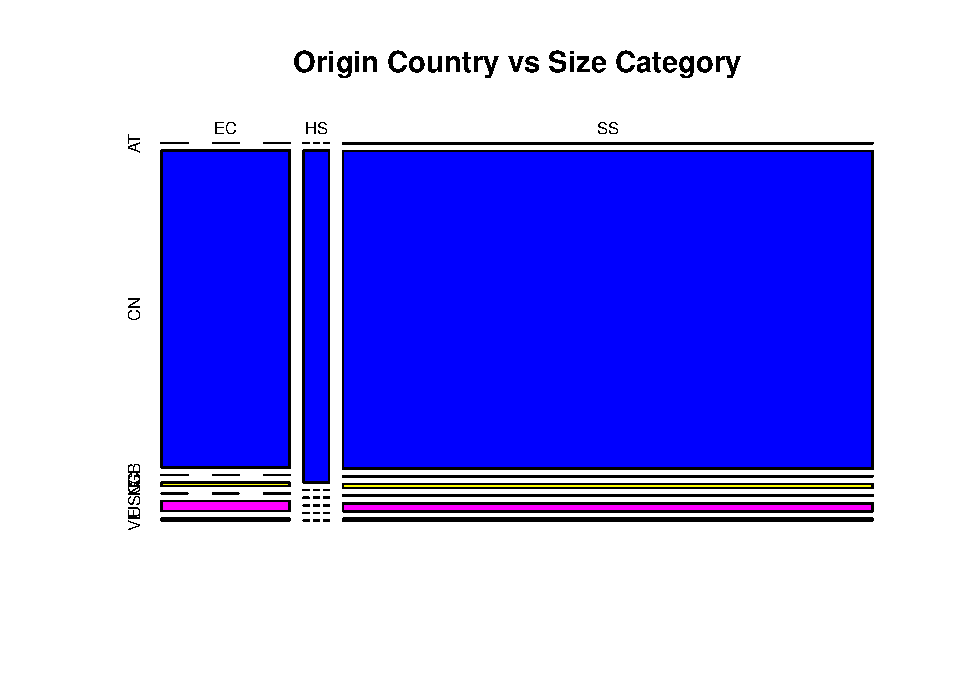
\includegraphics{PRAC2_Limpieza_Analisis_Datos---Sales_files/figure-latex/unnamed-chunk-52-1.pdf}

Vemos que la mayor contribución a los tipos de tallas viene de China,
especialmente sobre las tallas pequeñas. El siguiente país es Estados
Unidos, sobre todo en tallas pequeñas también. Hay una contribución de
ventas no catalogadas por país en las tallas grandes. Y países como
China que contribuyen en gran medida a ventas donde no se han indicado
las tallas.

\hypertarget{estudio-de-la-correlaciuxf3n-tests-chi-squared}{%
\section{2.4.4.4.2 Estudio de la Correlación / Tests
Chi-Squared}\label{estudio-de-la-correlaciuxf3n-tests-chi-squared}}

Estamos tratando variables cuantitativas politómicas y nominales, por lo
que, para valorar la independencia, el test Chi-squared resulta adecuado
en algunos casos, y el test exacto de Fisher en otros.

\begin{Shaded}
\begin{Highlighting}[]
\KeywordTok{chisq.test}\NormalTok{(Tabla.SC.OC)}
\end{Highlighting}
\end{Shaded}

\begin{verbatim}
## Warning in chisq.test(Tabla.SC.OC): Chi-squared approximation may be incorrect
\end{verbatim}

\begin{verbatim}
## 
##  Pearson's Chi-squared test
## 
## data:  Tabla.SC.OC
## X-squared = 2.9685, df = 12, p-value = 0.9958
\end{verbatim}

\begin{Shaded}
\begin{Highlighting}[]
\KeywordTok{fisher.test}\NormalTok{(Tabla.SC.OC, }\DataTypeTok{conf.level =} \FloatTok{0.95}\NormalTok{, }\DataTypeTok{simulate.p.value =} \OtherTok{FALSE}\NormalTok{)}
\end{Highlighting}
\end{Shaded}

\begin{verbatim}
## 
##  Fisher's Exact Test for Count Data
## 
## data:  Tabla.SC.OC
## p-value = 0.9842
## alternative hypothesis: two.sided
\end{verbatim}

Como el \textbf{p-value es \textgreater{} 0.05} no podemos rechazar la
hipotésis nula, que indica independencia entre ambas variables. Por lo
tanto no existe correlación entre ellas.

\textbf{\emph{Cálculo del modelo}}

\begin{Shaded}
\begin{Highlighting}[]
\NormalTok{model.sizecategory.origincountry =}\StringTok{ }\KeywordTok{multinom}\NormalTok{(SalesSummerObj}\OperatorTok{$}\NormalTok{origin_country }\OperatorTok{~}\StringTok{ }
\NormalTok{SalesSummerObj}\OperatorTok{$}\NormalTok{size_category, }\DataTypeTok{data =}\NormalTok{ SalesSummerObj)}
\end{Highlighting}
\end{Shaded}

\begin{Shaded}
\begin{Highlighting}[]
\CommentTok{# Obtenemos el summary}

\KeywordTok{summary}\NormalTok{(model.sizecategory.origincountry)}
\end{Highlighting}
\end{Shaded}

\begin{verbatim}
## Call:
## multinom(formula = SalesSummerObj$origin_country ~ SalesSummerObj$size_category, 
##     data = SalesSummerObj)
## 
## Coefficients:
##    (Intercept) SalesSummerObj$size_categoryHS SalesSummerObj$size_categorySS
## CN   12.564006                      16.728615                      -5.904251
## GB   -6.920249                      -2.284379                       6.920151
## NC    8.021308                      -2.924827                      -5.718242
## SG   -6.920249                      -2.284379                       6.920151
## US    9.119283                      -4.310894                      -6.174407
## VE    7.325471                      -2.612316                      -5.939105
## 
## Std. Errors:
##    (Intercept) SalesSummerObj$size_categoryHS SalesSummerObj$size_categorySS
## CN  38.9698400                   3.384340e-06                     38.9826651
## GB   0.7252816                   2.476857e-10                      0.7225532
## NC  38.9761825                   4.656710e-08                     38.9902715
## SG   0.7252816                   3.540281e-10                      0.7225532
## US  38.9719101                   1.137314e-08                     38.9853932
## VE  38.9826268                   6.407023e-08                     38.9986379
## 
## Residual Deviance: 472.4827 
## AIC: 508.4827
\end{verbatim}

\begin{Shaded}
\begin{Highlighting}[]
\CommentTok{# Coefcientes Modelo }

\NormalTok{coefmodel.sizecategory.origincountry <-}\StringTok{ }\KeywordTok{coef}\NormalTok{(model.sizecategory.origincountry)}

\NormalTok{coefmodel.sizecategory.origincountry}
\end{Highlighting}
\end{Shaded}

\begin{verbatim}
##    (Intercept) SalesSummerObj$size_categoryHS SalesSummerObj$size_categorySS
## CN   12.564006                      16.728615                      -5.904251
## GB   -6.920249                      -2.284379                       6.920151
## NC    8.021308                      -2.924827                      -5.718242
## SG   -6.920249                      -2.284379                       6.920151
## US    9.119283                      -4.310894                      -6.174407
## VE    7.325471                      -2.612316                      -5.939105
\end{verbatim}

Vamos a evaluar ahora los \textbf{\emph{odds ratio}}. Los
\textbf{\emph{odds}} es la razón de la probabilidad de ocurrencia de un
suceso entre la probabilidad de su no ocurrencia. Vamos a ver cómo
transformamos los coeficientes en odds ratios. Trataremos de ser algo
didácticos, y vamos a explicar en detalle su cálculo para China:

En esta expresión, el modelo está expresado en términos del
\textbf{\emph{log-odds}}:

\[
ln({\frac{P(Y=1/X)}{1-P(Y=1/X)}}) = 12.564 + 16.729 * HS  - 5.904 * SS
\] Si se escribe en términos de odds, se tiene:

\[
{\frac{P(Y=1/X)}{1-P(Y=1/X)}} = {\frac{e^{b_0}+ \sum_{i= 1}^{n}(b_{i}x_{i})}{1+e^{b_0}+\sum_{i= 1}^{n}(b_{i}x_{i})}}
\] Se calculan los distintos valores de las probabilidades para las
cuatro combinaciones entre la variable dependiente Y con la
independiente X:

\[
{\frac{P(Y=1/X=1)}{1-P(Y=1/X=1)}} = {\frac{e^{b_0+b_1}}{1+e^{b_0+b_1}}}
\]

\[
{\frac{P(Y=1/X=0)}{1-P(Y=1/X=0)}} = {\frac{e^{b_0}}{1+e^{b_0}}}
\]

\[
{\frac{P(Y=0/X=1)}{1-P(Y=0/X=1)}} = {\frac{1}{1+e^{b_0+b_1}}}
\]

\[
{\frac{P(Y=0/X=0)}{1-P(Y=0/X=0)}} = {\frac{1}{1+e^{b_0}}}
\]

Los \textbf{\emph{odds-ratio (OR)}} se calculan como la razón entre los
\textbf{\emph{odds}}, donde la variable respuesta Y está presente entre
los individuos, es decir, toma el valor Y = 1, y la variable
independiente X puede estar presente o no, es decir, tomar los valores X
= 1 y X = 0.

\[
OR = {\frac{{\frac{P(Y=1/X=1)}{1-P(Y=1/X=1)}}}{{\frac{P(Y=1/X=0)}{1-P(Y=1/X=0)}}}} = {e^{b_1}}
\]

• Un OR = 1 implica que no existe asociación entre la variable respuesta
y la covariable. • Un OR inferior a la unidad se interpreta como un
factor de protección, es decir, el suceso es menos probable en presencia
de dicha covariable. • Un OR mayor a la unidad se interpreta como un
factor de riesgo, es decir,el suceso es más probable en presencia de
dicha covariable.

Para el caso de los Estados Unidos:

\[
ln({\frac{P(Y=1/X)}{1-P(Y=1/X)}}) = 9.112 -4.31 * HS - 6.174 * SS 
\]

\begin{Shaded}
\begin{Highlighting}[]
\CommentTok{# Odds Ratios Modelo }

\KeywordTok{exp}\NormalTok{(coefmodel.sizecategory.origincountry)}
\end{Highlighting}
\end{Shaded}

\begin{verbatim}
##     (Intercept) SalesSummerObj$size_categoryHS SalesSummerObj$size_categorySS
## CN 2.860740e+05                   1.841388e+07                   2.727823e-03
## GB 9.875841e-04                   1.018372e-01                   1.012472e+03
## NC 3.045158e+03                   5.367396e-02                   3.285483e-03
## SG 9.875841e-04                   1.018372e-01                   1.012472e+03
## US 9.129652e+03                   1.342154e-02                   2.082040e-03
## VE 1.518489e+03                   7.336442e-02                   2.634386e-03
\end{verbatim}

Calcularemos ahora los intervalos de confianza:

\begin{Shaded}
\begin{Highlighting}[]
\CommentTok{# Intervalos de confianza odds ratio}


\NormalTok{Modelo.sizecategory.origincountry <-}\StringTok{ }\KeywordTok{confint}\NormalTok{(model.sizecategory.origincountry)}

\NormalTok{Modelo.sizecategory.origincountry}
\end{Highlighting}
\end{Shaded}

\begin{verbatim}
## , , CN
## 
##                                    2.5 %   97.5 %
## (Intercept)                    -63.81548 88.94349
## SalesSummerObj$size_categoryHS  16.72861 16.72862
## SalesSummerObj$size_categorySS -82.30887 70.50037
## 
## , , GB
## 
##                                    2.5 %    97.5 %
## (Intercept)                    -8.341775 -5.498723
## SalesSummerObj$size_categoryHS -2.284379 -2.284379
## SalesSummerObj$size_categorySS  5.503972  8.336329
## 
## , , NC
## 
##                                     2.5 %    97.5 %
## (Intercept)                    -68.370606 84.413222
## SalesSummerObj$size_categoryHS  -2.924827 -2.924827
## SalesSummerObj$size_categorySS -82.137770 70.701286
## 
## , , SG
## 
##                                    2.5 %    97.5 %
## (Intercept)                    -8.341775 -5.498723
## SalesSummerObj$size_categoryHS -2.284379 -2.284379
## SalesSummerObj$size_categorySS  5.503972  8.336329
## 
## , , US
## 
##                                     2.5 %    97.5 %
## (Intercept)                    -67.264257 85.502823
## SalesSummerObj$size_categoryHS  -4.310894 -4.310894
## SalesSummerObj$size_categorySS -82.584374 70.235559
## 
## , , VE
## 
##                                     2.5 %    97.5 %
## (Intercept)                    -69.079074 83.730015
## SalesSummerObj$size_categoryHS  -2.612316 -2.612316
## SalesSummerObj$size_categorySS -82.375031 70.496821
\end{verbatim}

\hypertarget{representaciuxf3n-de-resultados}{%
\section{2.5 - REPRESENTACIÓN DE
RESULTADOS}\label{representaciuxf3n-de-resultados}}

\textbf{Interpretación de Modelos}

\textbf{\emph{Vamos a representar gráficamente los datos de los
regresores retprice, pvinventory y ratingone respecto a price:}}

\begin{Shaded}
\begin{Highlighting}[]
\KeywordTok{scatter3D}\NormalTok{(}\DataTypeTok{x=}\NormalTok{retprice, }\DataTypeTok{y=}\NormalTok{pvinventory, }\DataTypeTok{z =}\NormalTok{ratingone ,}\DataTypeTok{groups=}\NormalTok{artprice, }\DataTypeTok{theta=}\DecValTok{30}\NormalTok{, }\DataTypeTok{phi=}\DecValTok{8}\NormalTok{, }\DataTypeTok{pch=}\DecValTok{20}\NormalTok{, }\DataTypeTok{bty =} \StringTok{"g"}\NormalTok{, }
          \DataTypeTok{grid=}\OtherTok{FALSE}\NormalTok{, }\DataTypeTok{fit=}\StringTok{"smooth"}\NormalTok{)}
\end{Highlighting}
\end{Shaded}

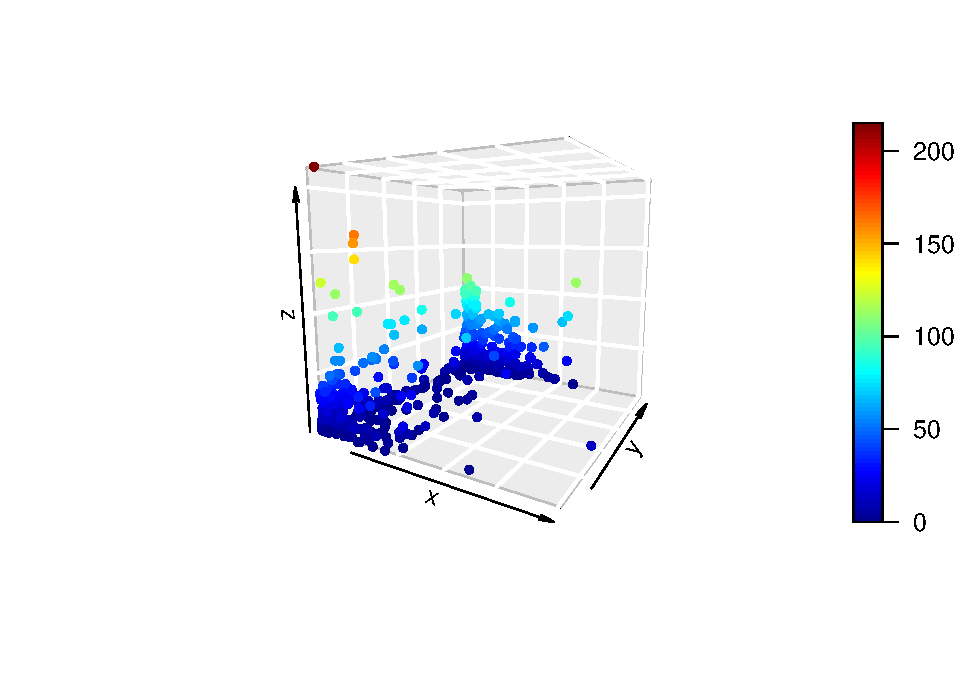
\includegraphics{PRAC2_Limpieza_Analisis_Datos---Sales_files/figure-latex/unnamed-chunk-61-1.pdf}

Vemos que los precios más bajos se concentran para valores bajos y altos
de inventario de la talla de la compra, y para precios de retail bajos.
Los precios medios se agrupan en los valores centrales de los tres
regresores, y los precios más altos se encuentran para valores bajos de
los regresores retprice y pvinventory, y para valores altos del regresor
ratingone.

\textbf{Tabla resumen modelo regresión logística multinomial}

\hypertarget{resoluciuxf3n-del-problema}{%
\section{2.6 - RESOLUCIÓN DEL
PROBLEMA}\label{resoluciuxf3n-del-problema}}

\hypertarget{referencias}{%
\section{REFERENCIAS}\label{referencias}}

Documentación máster UOC: Modelos\_de\_Regresión\_Logística.pdf
(PID\_00276229)

6 Errores que cometes al usar las pruebas de hipótesis clásicas:
\url{https://www.maximaformacion.es/blog-dat/6-errores-que-cometes-al-usar-las-pruebas-de-hipotesis-clasicas/}

Modelos con Variables Cualitativas:
\url{https://bookdown.org/content/2274/modelos-con-variables-cualitativas.html}

Estadística conceptos clave:
\url{https://www.usj.es/sites/default/files/tarjetas/aprendizaje/EstadisticaConceptosClave.pdf}

Análisis de variables categóricas con R:
\url{https://biocosas.github.io/R/060_analisis_datos_categoricos.html}

Correlación: teoría y práctica:
\url{https://www.ccg.unam.mx/~vinuesa/R4biosciences/docs/Tema8_correlacion.html}

Test estadísticos para variables cualitativas: test exacto de Fisher,
chi-cuadrado de Pearson, McNemar y Q-Cochran:
\url{https://www.cienciadedatos.net/documentos/22.2_test_exacto_de_fisher_chi-cuadrado_de_pearson_mcnemar_qcochran\#(chi\%5E2)_de_Pearson_(test_de_independencia)}

Logistic Regression in R: \url{https://rpubs.com/rslbliss/r_logistic_ws}

Multinomial distribution:
\url{https://en.wikipedia.org/wiki/Multinomial_distribution}

Test estadísticos para variables cualitativas: test binomial exacto,
test multinomial y test chi-cuadrado goodnes of
fit:\url{https://www.cienciadedatos.net/documentos/22.1_test_binomial_exacto_test_multinomial_test_chi-cuadrado_goodnes_of_fit}

Modelos de respuesta multinomial con R. Aplicación para el estudio de la
depresión en pacientes con discapacidad:
\url{https://masteres.ugr.es/moea/pages/tfm1011/modelosderespuestamultinomialconraplicacionparaelestudiodeladepresionenpacientescondiscapacidad/}!

Regresión Logística Multinomial:
Multinomialhttp://halweb.uc3m.es/esp/Personal/personas/jmmarin/esp/Categor/Tema5Cate.pdf
(Modelos Logit para respuestas nominales)

\end{document}
